\documentclass[a4paper,11pt]{book}
%\documentclass[a4paper,twoside,11pt,titlepage]{book}
\usepackage{listings}
\usepackage[utf8]{inputenc}
\usepackage[spanish]{babel}

%% Allows 'H' property in images, which makes possible
%% to force an image into a certain position
\usepackage{float}

%% In order to crop images
\usepackage{graphicx}

\usepackage[nottoc]{tocbibind}

\decimalpoint
\usepackage{dcolumn}
\newcolumntype{.}{D{.}{\esperiod}{-1}}
\makeatletter
\addto\shorthandsspanish{\let\esperiod\es@period@code}
\makeatother


%\usepackage[chapter]{algorithm}
\RequirePackage{verbatim}
%\RequirePackage[Glenn]{fncychap}
\usepackage{fancyhdr}
\usepackage{graphicx}
\usepackage{afterpage}

\usepackage{longtable}

\usepackage[hidelinks=true,pdfborder={000}]{hyperref} %referencia
\newcommand{\MYhref}[3][blue]{\href{#2}{\color{#1}{#3}}}%

% ********************************************************************
% Re-usable information
% ********************************************************************
\newcommand{\myTitle}{Desarrollo de un videojuego para la configuración y análisis de redes de computadores\xspace}
\newcommand{\myDegree}{Grado en Ingeniería de Tecnologías de Telecomunicación\xspace}
\newcommand{\myName}{Ángel Oreste Rodríguez Romero\xspace}
\newcommand{\myProf}{Juan José Ramos Muñoz\xspace}
\newcommand{\myOtherProf}{Jonathan Prados Garzón\xspace}
%\newcommand{\mySupervisor}{Put name here\xspace}
\newcommand{\myFaculty}{Escuela Técnica Superior de Ingenierías Informática y de
Telecomunicación\xspace}
\newcommand{\myFacultyShort}{E.T.S. de Ingenierías Informática y de
Telecomunicación\xspace}
\newcommand{\myDepartment}{Departamento de TSTC\xspace}
\newcommand{\myUni}{\protect{Universidad de Granada}\xspace}
\newcommand{\myLocation}{Granada\xspace}
\newcommand{\myTime}{\today\xspace}
\newcommand{\myVersion}{Version 0.1\xspace}

%% My commands
\newcommand{\GNSCS}{\texttt{GNS3sharp}}
\newcommand{\NODE}{\texttt{Node}}
\newcommand{\LINK}{\texttt{Link}}
\newcommand{\GAOBJ}{\texttt{GameObject}}


\hypersetup{
pdfauthor = {\myName (aoreste96@correo.ugr.es)},
pdftitle = {\myTitle},
pdfsubject = {},
pdfkeywords = {GNS3, Unity, telemática, API, ...},
pdfcreator = {LaTeX con el paquete ....},
pdfproducer = {pdflatex}
}

%\hyphenation{}


%\usepackage{doxygen/doxygen}
%\usepackage{pdfpages}
\usepackage{url}
\usepackage{colortbl,longtable}
\usepackage[stable]{footmisc}
%\usepackage{index}

%\makeindex
%\usepackage[style=long, cols=2,border=plain,toc=true,number=none]{glossary}
% \makeglossary

% Definición de comandos que me son tiles:
%\renewcommand{\indexname}{Índice alfabético}
%\renewcommand{\glossaryname}{Glosario}

\pagestyle{fancy}
\fancyhf{}
\fancyhead[LO]{\leftmark}
\fancyhead[RE]{\rightmark}
\fancyhead[RO,LE]{\textbf{\thepage}}
\renewcommand{\chaptermark}[1]{\markboth{\textbf{#1}}{}}
\renewcommand{\sectionmark}[1]{\markright{\textbf{\thesection. #1}}}

\setlength{\headheight}{1.5\headheight}

\newcommand{\HRule}{\rule{\linewidth}{0.5mm}}
%Definimos los tipos teorema, ejemplo y definición podremos usar estos tipos
%simplemente poniendo \begin{teorema} \end{teorema} ...
\newtheorem{teorema}{Teorema}[chapter]
\newtheorem{ejemplo}{Ejemplo}[chapter]
\newtheorem{definicion}{Definición}[chapter]

\definecolor{gray97}{gray}{.97}
\definecolor{gray75}{gray}{.75}
\definecolor{gray45}{gray}{.45}
\definecolor{gray30}{gray}{.94}

\lstset{ frame=Ltb,
     framerule=0.5pt,
     aboveskip=0.5cm,
     framextopmargin=3pt,
     framexbottommargin=3pt,
     framexleftmargin=0.1cm,
     framesep=0pt,
     rulesep=.4pt,
     backgroundcolor=\color{gray97},
     rulesepcolor=\color{black},
     %
     stringstyle=\ttfamily,
     showstringspaces = false,
     basicstyle=\scriptsize\ttfamily,
     commentstyle=\color{gray45},
     keywordstyle=\bfseries,
     %
     numbers=left,
     numbersep=6pt,
     numberstyle=\tiny,
     numberfirstline = false,
     breaklines=true,
   }
 
% minimizar fragmentado de listados
\lstnewenvironment{listing}[1][]
   {\lstset{#1}\pagebreak[0]}{\pagebreak[0]}

\lstdefinestyle{CodigoCs}
   {
	basicstyle=\scriptsize,
	frame=single,
	language=csh,
	numbers=none
   }
 
\lstdefinestyle{Consola}
   {basicstyle=\scriptsize\bf\ttfamily,
    backgroundcolor=\color{gray30},
    frame=single,
    numbers=none
   }


\newcommand{\bigrule}{\titlerule[0.5mm]}


%Para conseguir que en las páginas en blanco no ponga cabecerass
\makeatletter
\def\clearpage{%
  \ifvmode
    \ifnum \@dbltopnum =\m@ne
      \ifdim \pagetotal <\topskip
        \hbox{}
      \fi
    \fi
  \fi
  \newpage
  \thispagestyle{empty}
  \write\m@ne{}
  \vbox{}
  \penalty -\@Mi
}
\makeatother

\usepackage{pdfpages}


%%%%%%%%%%%%%%%%%%%%%%%%%%%%%%%%%%%%%%%%%%%%
\begin{document}
% 0. Portada y prefacio
\begin{titlepage}
 
 
\newlength{\centeroffset}
\setlength{\centeroffset}{-0.5\oddsidemargin}
\addtolength{\centeroffset}{0.5\evensidemargin}
\thispagestyle{empty}

\noindent\hspace*{\centeroffset}\begin{minipage}{\textwidth}

\centering
\includegraphics[width=0.9\textwidth]{imagenes/logo_ugr.jpg}\\[1.4cm]

\textsc{ \Large TRABAJO FIN DE GRADO\\[0.2cm]}
\textsc{INGENIERÍA DE TECNOLOGÍAS DE TELECOMUNICACIÓN}\\[1cm]
% Upper part of the page
% 
% Title
{\Large\bfseries Desarrollo de un videojuego para la configuración y análisis de redes de computadores\\
}
\noindent\rule[-1ex]{\textwidth}{3pt}\\[3.5ex]
{\large\bfseries GNS3sharp}
\end{minipage}

\vspace{2.5cm}
\noindent\hspace*{\centeroffset}\begin{minipage}{\textwidth}
\centering

\textbf{Autor}\\ {Ángel Oreste Rodríguez Romero}\\[2.5ex]
\textbf{Directores}\\
{Juan José Ramos Muñoz\\
Jonathan Prados Garzón}\\[2cm]
\includegraphics[width=0.3\textwidth]{imagenes/etsiit_logo.png}\\[0.1cm]
\textsc{Escuela Técnica Superior de Ingenierías Informática y de Telecomunicación}\\
\textsc{---}\\
Granada, agosto de 2018
\end{minipage}
%\addtolength{\textwidth}{\centeroffset}
%\vspace{\stretch{2}}
\end{titlepage}



\chapter*{}
%\thispagestyle{empty}
%\cleardoublepage

%\thispagestyle{empty}

\begin{titlepage}
 
 
\setlength{\centeroffset}{-0.5\oddsidemargin}
\addtolength{\centeroffset}{0.5\evensidemargin}
\thispagestyle{empty}

\noindent\hspace*{\centeroffset}\begin{minipage}{\textwidth}

\centering
%\includegraphics[width=0.9\textwidth]{imagenes/logo_ugr.jpg}\\[1.4cm]



 \vspace{3.3cm}

%si el proyecto tiene logo poner aquí
\includegraphics[scale=0.5]{imagenes/logo.png} 
 \vspace{0.5cm}

% Title

{\Huge\bfseries Desarrollo de un videojuego para la configuración y análisis de redes de computadores\\
}
\noindent\rule[-1ex]{\textwidth}{3pt}\\[3.5ex]
{\large\bfseries GNS3sharp\\[4cm]}
\end{minipage}

\vspace{2.5cm}
\noindent\hspace*{\centeroffset}\begin{minipage}{\textwidth}
\centering

\textbf{Autor}\\ {Ángel Oreste Rodríguez Romero}\\[2.5ex]
\textbf{Directores}\\
{Juan José Ramos Muñoz\\
Jonathan Prados Garzón}\\[2cm]
%\includegraphics[width=0.15\textwidth]{imagenes/tstc.png}\\[0.1cm]
%\textsc{Departamento de Teoría de la Señal, Telemática y Comunicaciones}\\
%\textsc{---}\\
%Granada, mes de 201
\end{minipage}
%\addtolength{\textwidth}{\centeroffset}
\vspace{\stretch{2}}

 
\end{titlepage}






\cleardoublepage
\thispagestyle{empty}

\begin{center}
{\large\bfseries Desarrollo de un videojuego para la configuración y análisis de redes de computadores: GNS3sharp}\\
\end{center}
\begin{center}
Ángel Oreste Rodríguez Romero\\
\end{center}

%\vspace{0.7cm}
\noindent{\textbf{Palabras clave}: palabra\_clave1, palabra\_clave2, palabra\_clave3, ......}\\

\vspace{0.7cm}
\noindent{\textbf{Resumen}}\\

El jugar ha sido desde siempre un gran amigo de la educación. Aprender jugando es un lema que cada vez se repite más. Los videojuegos, concretamente, toman en cierta forma el relevo de los juegos tal y como tradicionalmente estos se han entendido y amplían sus posibilidades.

La era digital afecta a casi todos los ámbitos de nuestro entorno. Las redes no iban a quedar excluidas de ese avance. Así, se pueden encontrar decenas de implementaciones virtuales de redes de telecomunicaciones, permitiéndonos visualizar su funcionamiento evitando el desembolso que equivale una real.

Digitalizados ambos ámbitos, ¿por qué no unirlos? ¿Y por qué no unirlos con un propósito educacional?

El presente documento pretende realizar un acercamiento a tal propósito. Se listará una serie de tecnologías que permiten llevar esto a cabo así como el desarrollo de mi aproximación.
\cleardoublepage


\thispagestyle{empty}


\begin{center}
{\large\bfseries Development of a videogame for the configuration and analysis of computer networks: GNS3sharp}\\
\end{center}
\begin{center}
Ángel Oreste, Rodríguez Romero\\
\end{center}

%\vspace{0.7cm}
\noindent{\textbf{Keywords}: Keyword1, Keyword2, Keyword3, ....}\\

\vspace{0.7cm}
\noindent{\textbf{Abstract}}\\

Playing has always been a great friend of education. Learning by playing is a motto that is repeated more and more. Videogames, in particular, take over from games as they have traditionally been understood and expand their possibilities.

The digital age affects almost every area of our environment. Networks would not be excluded from this development. Thus, dozens of virtual implementations of telecommunication networks can be found, allowing us to visualize them working, avoiding the disbursement that is equivalent to a real one.

Digitized both areas, why not unite them, and why not unite them for an educational purpose?

This document is intended to bring this about. A number of technologies will be listed that allow this to be done as well as the development of my approach.

\chapter*{}
\thispagestyle{empty}

\noindent\rule[-1ex]{\textwidth}{2pt}\\[4.5ex]

Yo, \textbf{Ángel Oreste Rodríguez Romero}, alumno de la titulación Ingeniería de Tecnologías de Telecomunicación de la \textbf{Escuela Técnica Superior
de Ingenierías Informática y de Telecomunicación de la Universidad de Granada}, con DNI 25351379C, autorizo la
ubicación de la siguiente copia de mi Trabajo Fin de Grado en la biblioteca del centro para que pueda ser
consultada por las personas que lo deseen.

\vspace{6cm}

\noindent Fdo: Ángel Oreste Rodríguez Romero

\vspace{2cm}

\begin{flushright}
Granada a 1 de septiembre de 2018.
\end{flushright}


\chapter*{}
\thispagestyle{empty}

\noindent\rule[-1ex]{\textwidth}{2pt}\\[4.5ex]

D. \textbf{Juan José Ramos Muñoz}, Profesor del Área de Telemática del Departamento TSTC de la Universidad de Granada.

\vspace{0.5cm}

D. \textbf{Jonathan Prados Garzón}, Profesor del Área de Telemática del Departamento TSTC de la Universidad de Granada.


\vspace{0.5cm}

\textbf{Informan:}

\vspace{0.5cm}

Que el presente trabajo, titulado \textit{\textbf{Desarrollo de un videojuego para la configuración y análisis de redes de computadores: GNS3sharp}},
ha sido realizado bajo su supervisión por \textbf{Ángel Oreste Rodríguez Romero}, y autorizamos la defensa de dicho trabajo ante el tribunal
que corresponda.

\vspace{0.5cm}

Y para que conste, expiden y firman el presente informe en Granada a 1 de septiembre de 2018.

\vspace{1cm}

\textbf{Los directores:}

\vspace{5cm}

\noindent \textbf{Juan José Ramos Muñoz \ \ \ \ \ Jonathan Prados Garzón}

\chapter*{Agradecimientos}
\thispagestyle{empty}

       \vspace{1cm}

A Juanjo, por su increíble paciencia e inestimable ayuda, tanto en nuestras tutorías presenciales como aquellas improvisadas por Telegram. A todos esos profesores que confiaron en mí y en mis capacidades más que yo mismo en tantos momentos. A todos aquellos compañeros como Alfonso que no solo me facilitaron la vida académica con su conocimiento, sino también con su compañía. A Alberto, que aunque algo reticente de primeras, está dispuesto a echarme una mano de pedírselo. A mis compañeros de Francia, que me impulsaron a ampliar mis conocimientos. A Antonio por el logo tan genial que ha hecho. A mi grupo, porque sin él no habría tenido el ánimo suficiente durante este año para afrontar el proyecto. A todos aquellos amigos que me oyeron quejarme de mi proyecto con estoicismo. A la comunidad de StackOverflow que de tantos apuros me ha sacado.

Pero ante todo, a mis padres, pilar fundamental y soporte absoluto de toda mi vida, universitaria o no. Por la educación que me han dado, por todos aquellos caprichos que me permitieron y por velar siempre por mi salud.

% 0. Tablas de contenido
\frontmatter
\tableofcontents
%\listoffigures
%\listoftables

% Capítulos
\mainmatter
\setlength{\parskip}{5pt}
\chapter{Introducción}\label{chap:Intro}
Este primer capítulo introductorio sirve de acercamiento tanto al problema con el que se pretende resolver como al modo con el que se decidió resolverlo. Al final del mismo se listarán los distintos capítulos del documento así como un breve resumen de cada uno de ellos.

\section{Introducción}
El siguiente trabajo se propone desarrollar un \textbf{videojuego capaz de integrar un simulador de redes} en sus mecánicas; esto es, capaz de \textbf{verse afectado} por la configuración establecida en una red virtualizada y, a la misma vez, tener el poder de modificarla desde el propio juego. La finalidad de todo esto no reside en el entretenimiento puro que brinda el mundo del videojuego, sino en las puertas que abre para el mundo docente. Si consideramos a los videojuegos un medio para facilitar el aprendizaje, de hacerlo más atractivo al público, la integración de redes reales en ellos puede permitir crear un nuevo camino docente en el ámbito de las redes. Finalmente no es más que una forma de facilitar el aprendizaje para el mayor número de personas posible.

Se analizará una serie de tecnologías para seleccionar las más adecuadas para el trabajo. Como resultado de todo lo anterior, se proporcionará una biblioteca para que los desarrolladores puedan crear sus propios juegos sobre el simulador de red, y un juego de ejemplo de uso.

\subsection{Motivación}
\subsubsection{Los videojuegos y la educación}
Contrariamente al modelo educativo tradicional, en que el que la atención gira en torno al profesor, desde principios del nuevo milenio aparece el \textit{aprendizaje centrado en el estudiante}. Aunque el origen del concepto puede datarse a principios del siglo pasado, no ha sido hasta este que ha comenzado a tomar forma. Carl Rogers, en su libro ``Freedom to Learn for the 80s'', describe el cambio de poder del profesor experto al alumno, impulsado por la necesidad de un cambio en el entorno tradicional en el que, en esta "llamada atmósfera educativa, los estudiantes se vuelven pasivos, apáticos y aburridos"\cite{studentcentered}.

R.M Harden y Joy Crosby, en un artículo realizado en el 2000, describen las estrategias de aprendizaje centradas en el ``maestro'' desde el enfoque de \textit{el maestro que transmite el conocimiento}, del experto al principiante. En contraste, describen el aprendizaje centrado en el estudiante como aquel enfocado en el aprendizaje de los estudiantes y ``lo que los estudiantes hacen para lograrlo, en lugar de lo que hace el maestro''. Esta definición enfatiza el concepto del estudiante \textit{haciendo} \cite{goodteacher}.

Es aquí donde los videojuegos pueden ayudar. Este mismo año, un informe salía a la luz dando una serie de datos bastante interesantes al respecto. El informe, desarrollado por \href{https://triseum.com/}{Triseum} (empresa dedicada de lleno a los videojuegos educativos), es un proyecto europeo con el propósito de probar y evaluar el aprendizaje basado en juegos con dos videojuegos educativos (ambos juegos creados por la propia empresa del estudio). De entre los 20 profesores que llevaron a sus aulas los juegos, ninguno de ellos tuvo experiencias negativas con ellos. Algunos de los más satisfechos con la prueba contaban que ``los estudiantes estaban muy motivados y mucho mejor preparados para las siguientes asignaturas y conceptos de la clase, construidos mediante el contenido y los conceptos tratados en el juego''\cite{triseum}.

Son muchos los estudios que se han llevado a cabo con el fin de demostrar el potencial didáctico de los videojuegos. Algunos de ellos se han centrado en exponer el uso de juegos comerciales en escuelas \cite{gamesinclass}, y otros tantos  el de juegos nacidos por y para la educación \cite{edugamesinclass}. Todos entre aquellos en la bibliografía consultada, como el realizado por Kennedy-Clark y Thompson en 2011, concluyen que los beneficios de usar los videojuegos como método de aprendizaje funciona. Este último, asevera que ``como se encontró en muchos otros estudios, el mundo virtual fue motivador, interesante y atractivo para los estudiantes''\cite{deathrome}.

Y es que la virtualización es una herramienta enormemente versátil. Empresas como Labster se han dado cuenta de ello. Esta compañía se encarga de desarrollar laboratorios virtuales y propuestas lúdicas para la enseñanza de materias relacionadas con la ciencia, muchas de ellas llevadas a cabo en forma de videojuego\cite{labster}. ``Al integrar simulaciones en laboratorios virtuales permitimos que los alumnos tengan acceso ilimitado y económico y que practiquen todo lo que quieran hasta que aprendan los conceptos perfectamente'', dice su fundador, el danés Michael Bodekaer.	

\subsubsection{Enfoque del trabajo}
Es entonces nuestra misión llevar esto último al terreno de las telecomunicaciones. A sabiendas de que los videojuegos suponen un portal educativo de gran riqueza, nos proponemos desarrollar un ejemplo de \textbf{juego que permita aprender conceptos sobre telemática}.

La telemática ``describe los procesos de transmisión y gestión de informaciones digitales así como los servicios y aplicaciones que se apoyan en ellos''\cite{telematica}. Entre esos servicios se encuentran las redes de telecomunicaciones. La infraestructura asociada a estas suele ser cara y costosa, requiriendo un desembolso importante así como un despliegue inicial no apto para cualquiera. Esto recuerda directamente a las palabras anteriormente expuestas por el fundador de Labster. Su solución fue virtualizar laboratorios e insertarlos en juegos para, así, acercar estos a los estudiantes. Nosotros aquí pretendemos algo similar.

El fin que se propone este trabajo es el de crear un videojuego que integre una red virtualizada. Por suerte para nosotros, a diferencia de Bodekaer, no tenemos que encargarnos de crear un sistema de virtualización de redes, pues, como veremos con detalle en el capítulo \ref{chap:ArtState}, ya existen varios. El objetivo principal pasa por enlazar tal simulador de redes (una herramienta de virtualización de las mismas) con un videojuego.

Precisamente aquel es el primordial problema con el que se habrá de lidiar. A día de hoy, no existe forma directa de unir un videojuego con un simulador de redes. Hay que considerar que estos simuladores están concebidos como finalidad en sí mismos (como una aplicación cualquiera) y no como herramienta para ser usada por utilidades externas. Se requiere por consiguiente desarrollar una infraestructura que haga de nexo entre la red virtual y un videojuego.
 
\subsection{Objetivos}
Aclarado lo anterior, los objetivos que el proyecto se propone son los siguientes:
\begin{itemize}
\item Posibilitar la \textbf{interacción directa entre un videojuego y un simulador de redes}. Aquí reside nuestro papel fundamental del proceso. Con tal propósito crearemos una librería desde la que poder realizar la interacción.
\item \textbf{Desarrollar un videojuego} que haga uso de tal librería; que sea capaz, asimismo, de encontrar un uso didáctico para ella y aplicarlo.
\end{itemize}

\section{Estructura del trabajo}
Para finalizar el capítulo, se expondrá a modo de adelanto una lista que recoge cada capítulo a tratar en el proyecto. Junto a todos ellos, se incluye un pequeño resumen que pretende dar a conocer qué podrá estudiarse en sus respectivas páginas:
\begin{itemize}
\item \textbf{Capítulo \ref{chap:Intro}: Introducción}. En el actual capítulo, como ya se ha podido ver, se han abordado los distintas causas que han motivado a existir a este proyecto a la vez que la forma en la que se intentará llevar a buen puerto su resolución.
\item \textbf{Capítulo \ref{chap:Plan}: Planificación}. Una guía del trabajo llevado a cabo, concerniente tanto a la manera en que se ha distribuido temporalmente como a los utensilios empleados.
\item \textbf{Capítulo \ref{chap:ArtState}: Estado del arte}. Las distintas tecnologías barajadas sobre las que trabajar son aquí listadas.
\item \textbf{Capítulo \ref{chap:Analisis}: Análisis tecnológico}. Tras citar algunos ejemplos de tecnologías que podrían emplearse para el proyecto en el anterior capítulos, aquí se hace un análisis más en profundidad de las que han resultado escogidas.
\item \textbf{Capítulo \ref{chap:Design}: Diseño}. Se determina la forma en la que se llevará a cabo la solución del problema inicial.
\item \textbf{Capítulo \ref{chap:Integration}: Implementación}. Trazado un camino a seguir en el capítulo anterior, en este se describe la manera en la que este camino toma forma. Se muestra qué se ha creado finalmente y cómo se ha logrado.
\item \textbf{Capítulo \ref{chap:Pruebas}: Pruebas}. En este capítulo el resultado final es mostrado y se añade una valoración del mismo.
\item \textbf{Capítulo \ref{chap:Conclusiones}: Conclusiones}. Para finalizar el proyecto, se ha hecho un resumen del trabajo realizado junto a una valoración del mismo. Además, algunas propuestas de trabajos futuros sobre él son dadas.
\end{itemize}

\chapter{Planificación}\label{chap:Plan}

fgxdh

\section{Planificación temporal}

huigk

\section{Recursos empleados}
Dividiremos los recursos utilizados para la realización del trabajo en tres: recursos humanos, recursos software y recursos hardware:

\subsection{Recursos humanos}
Aquí una lista de las personas que han participado en el proyecto y su papel en el mismo.
\begin{itemize}
\item Juan José Ramos Muñoz, profesor del departamento de Teoría de
la Señal, Telemática y Comunicaciones en la ETSIIT de la Universidad de Granada. Tutor del proyecto
\item Jonathan Prados Garzón, profesor del departamento de Teoría de
la Señal, Telemática y Comunicaciones en la ETSIIT de la Universidad de Granada.
Cotutor del proyecto.
\item Ángel Oreste Rodríguez Romero, alumno del grado de ingeniería de tecnologías de telecomunicación en la ETSIIT de la Universidad de Granada. Autor del proyecto.
\end{itemize}

\subsection{Recursos software}
Aplicaciones y demás material digital que ha sido necesario para desarrollar el trabajo:
\begin{itemize}
\item \href{https://www.microsoft.com/es-es/windows}{\textbf{Microsoft Windows 10 Home versión 1803}} como sistema operativo sobre el que se ha llevado todo el proyecto a cabo.
\item Se usará además \href{https://xubuntu.org/about/}{\textbf{Xubuntu 18.04}} instalado en una máquina virtual para llevar ciertas pruebas del capítulo \ref{chap:Pruebas} a cabo.
\item \href{https://www.mozilla.org/es-ES/firefox/}{\textbf{Mozilla Firefox Quantum}} como navegador web. 61.0.2 es la última versión empleada.
\item Para la realización de la memoria:
\begin{itemize}
\item El editor \href{http://www.xm1math.net/texmaker/}{\textbf{Texmaker 5.0.2}} junto a \href{https://miktex.org/about}{MiKTeX 2.9}, implementación de \LaTeX.
\item \href{https://es.libreoffice.org/descubre/draw/}{\textbf{LibreOffice Draw 6.1.0.3}} para el diseño de algunos esquemas.
\item \href{https://inkscape.org/es/}{\textbf{InkScape 0.92}} para la transformación de imágenes vectoriales en archivos de formato \textit{.pdf}.
\end{itemize}
\item Como lector de archivos \textit{.pdf} ha sido elegido \href{https://www.foxitsoftware.com/pdf-reader/}{\textbf{Foxit Reader}}. Última versión: 9.2.0.
\item Para el desarrollo de código:
\begin{itemize}
\item El editor más utilizado durante el transcurso del trabajo ha sido \href{https://code.visualstudio.com/}{\textbf{Visual Studio Code}}. Ha pasado por varias versiones durante su uso. La más reciente es 1.26.
\item Para la compilación de código y el scripting en Unity el hermano mayor del anterior, \href{https://visualstudio.microsoft.com/es/}{\textbf{Microsoft Visual Studio}}, también ha pasado por varias versiones, pero la última de ellas ha sido la 15.8.0.
\item \href{https://notepad-plus-plus.org/}{\textbf{Notepad++}} ha sido utilizado para tomar notas y revisar código de forma rápida y ligera. La última versión usada es la 7.5.8.
\item \href{https://www.visual-paradigm.com/}{Visual Paradigm Enterprise 15.1} para dibujar los diagramas UML.
\end{itemize}
\item Para la virtualización de redes:
\begin{itemize}
\item \href{https://www.gns3.com/}{\textbf{GNS3 2.1.3 y finalmente 2.1.9}} como simulador de redes.
\item \href{https://www.virtualbox.org/}{\textbf{VirtualBox 5.2.16}} para la virtualización de ciertos dispositivos de la red y la instalación de un sistema Linux (Xubuntu) en el que integrar GNS3.
\end{itemize}
\item El motor para el desarrollo de videojuegos \href{https://unity3d.com/es}{\textbf{Unity}} versión personal. El último número de versión empleado ha sido el 2018.2.2f1.
\item Para el capítulo \ref{chap:Pruebas} serán útil \href{https://docs.microsoft.com/en-us/sysinternals/downloads/rammap}{\textbf{RamMap 1.51}} y \href{https://docs.microsoft.com/en-us/sysinternals/downloads/process-explorer}{\textbf{Process Explorer 16.21}}.
\end{itemize}

\subsection{Recursos hardware}
Todo el proyecto ha sido construido a través del portátil Lenovo Z500. Cuenta con un procesador Intel i7 3232QM de ocho núcleos virtuales, 16GB de RAM DDR3 a 798MHz, un disco duro HDD de 1GB a 5400RPM y una tarjeta gráfica dedicada Nvidia 740M con 1GB VRAM.

\section{Presupuesto}




\chapter{Estado del arte}\label{chap:ArtState}

El estado del arte se define como el nivel de desarrollo de un ámbito concreto, generalmente relacionado con el mundo técnico-científico. Este capítulo se encarga de hacer un listado de aquellas tecnologías que podrían sernos útiles así como de dar una serie de apuntes acerca de cada una de ellas. Dividiremos las tecnologías en dos grandes secciones: simuladores/emuladores de red y motores de videojuego.

\section{Simuladores y emuladores de red}\label{sec:simuladoremulador}
Un simulador de red es un software que predice el comportamiento de una red de datos. En los simuladores, la red se modela con dispositivos, enlaces, aplicaciones, etc. y se informa del rendimiento de la red. La mayoría de los simuladores utilizan la simulación de eventos discretos (modelado de sistemas en los que las variables de estado cambian en momentos discretizados de tiempo). El comportamiento de la red y las diversas aplicaciones y servicios que soporta pueden ser observados en un laboratorio de pruebas; varios atributos del entorno también pueden ser modificados de manera controlada para evaluar cómo se comportarían la red bajo diferentes condiciones \cite{wiki:Network_simulation}.

Sin embargo, conviene no confundir ``simuladores'' con ``emuladores'' de red. Un simulador puede realizar tareas replicadas para demostrar el comportamiento de una red y sus componentes, mientras que un emulador puede copiar el comportamiento de una red para reemplazarla funcionalmente \cite{emsim}.

En un nivel básico, un simulador de red utiliza fórmulas matemáticas para crear un modelo teórico y totalmente virtual de una red. Los simuladores son soluciones software. Si bien se utilizan principalmente con fines de investigación y educación, también pueden actuar como herramientas de prueba cruciales en el diseño y desarrollo de una red. Nosotros mostraremos ejemplos de ambos indistintamente. Solo citaremos aquellos gratuitos y/o open source.

\subsection{Mininet}
\textbf{Mininet} es un emulador de red que crea una red de hosts virtuales, switches, controladores y enlaces. Utiliza la virtualización basada en procesos de forma que es capaz de ejecutar muchos nodos (según la web, ha logrado levantar incluso 4096 a la vez) en un único núcleo del sistema operativo. Desde su versión 2.2.26, Linux soporta \texttt{namespace}s de red, una característica de virtualización ligera que proporciona a los procesos individuales interfaces de red separadas, tablas de enrutamiento y tablas ARP (del inglés, \textit{Address Resolution Protocol}). Mininet puede crear switches OpenFlow en el kernel o en el espacio de usuario, controladores para controlar los conmutadores y hosts para comunicarse a través de la red simulada. Se encarga de conectarlos usando pares de ethernet virtual (\texttt{veth})\cite{mininet}.

Mininet presenta una serie de ventajas muy interesantes en el mundo de la virtualización de redes:
\begin{itemize}
\item Capacidad de alojamiento de miles de dispositivos en una misma red. 
\item Asegura un arranque rápido de los nodos.
\item Tiene una instalación muy sencilla, pues es posible descargarse desde su web máquinas virtuales con todo preparado para que tan solo sea necesario instalarla en un hipervisor. También admite instalación nativa para Linux.
\item Cuenta con una \MYhref{http://mininet.org/api/annotated.html}{API} (del inglés, \textit{Application Programming Interface} desde la que poder interactuar con la red y los dispositivos desplegados en ella. Sin embargo, está escrita en Python y no hemos dado con ningún motor de videojuegos que admita a este como lenguaje de scripting nativo.
\item También posee una interfaz de usuario desde la que construir y gestionar la red.
\end{itemize}

Los últimos commits del \MYhref{https://github.com/mininet/mininet}{repositorio de Mininet} son anteriores al último mes, con lo que es claro que el proyecto sigue siendo mantenido.

\subsection{Common Open Research Emulator (CORE)}
\textbf{CORE} es una herramienta para construir redes virtuales. Como emulador, construye una representación de una red telemática real que funciona en tiempo real, a diferencia de la simulaciones de red, en las que como ya vimos se utilizan modelos abstractos.  La emulación en vivo puede conectarse a redes físicas y routers. Proporciona un entorno para ejecutar aplicaciones y protocolos reales, aprovechando las ventajas de la virtualización proporcionada por Linux o FreeBSD, únicos sistemas operativos donde está disponible. 

Algunas de sus características clave son:
\begin{itemize}
\item Es eficiente y escalable.
\item Ejecuta aplicaciones y protocolos reales sin modificaciones.
\item Cuenta con una interfaz gráfica de usuario fácil de usar.
\item Es altamente personalizable.
\end{itemize}

CORE se utiliza típicamente para la investigación de redes y protocolos, demostraciones, pruebas de aplicaciones y plataformas, evaluación de escenarios de redes, estudios de seguridad y aumento del tamaño de las redes físicas de prueba. Permite la inclusión de otras tecnologías de emulación de red como EMANE y ns-3 \cite{core}.

Sus características fundamentales son similares a las del emulador previamente citado. Al igual que aquel, CORE puede ser usado a través del GUI (la interfaz de usuario) o scripting mediante Python. Además, cuenta con una API propia. El demonio de Linux que CORE levanta escucha en un socket TCP para los mensajes de la API que lleguen de otra aplicación local o remota. La interfaz de usuario de CORE se conecta localmente a este demonio y utiliza la API para instanciar topologías. CORE también actuará como una ``servidor de emulación'' que escucha conexiones TCP de otro sistema. En el momento de la conexión, el otro sistema transmite mensajes al demonio de CORE, el cual puede controlar la la emulación en tiempo real \cite{coreapi}.

\subsection{GNS3}
GNS3 es un simulador gráfico de red multiplataforma \href{https://github.com/GNS3}{open-source} que se ejecuta en Windows, macOS y Linux \cite{bookgns}. Esto ya presenta una cierta ventaja respecto a sus anteriores competidores, cuya instalación solo es posible en Linux (y FreeBSD en el caso de CORE). Permite la virtualización de dispositivos reales tales como routers Cisco (para lo cual está especialmente preparado) y conectividad con otras redes reales como internet. Según su web, algunas de las marcas que utilizan este software son at\&t, Intel, NASA o Verizon \cite{gnsweb}.

La aplicación crea un servidor en la máquina en la que es lanzado al cual se puede acceder mediante una API REST. 

Cuenta con \MYhref{https://docs.gns3.com/}{documentación online}, \MYhref{https://gns3.com/community}{foros muy activos} e incluso una \MYhref{https://academy.gns3.com/}{academia} donde se imparten cursos.  

En el capítulo \ref{chap:Analisis} hablaremos con más detenimiento de este simulador.

\subsection{Más simuladores/emuladores}
Existen más aplicaciones que virtualizan redes que no explicaremos aquí. Por citar algunas: Cloonix, Netkit, Shadow, VNX...


\section{Motores de juego}
Un motor de juego proporciona multitud de características que son útiles a través de muchos juegos diferentes, por lo que un juego implementado con ese motor obtiene todas esas características junto a elementos artísticos personalizados y código de juego específico para él \cite{unityinaction}. 

Dividiremos cada uno de los que veremos en tres secciones fundamentales: plataformas hacia donde los juegos pueden ser exportados, características, lenguajes de programación que usan y precio.

\subsection{Unreal Engine}
Con una lista inmensa de juegos desarrollados con él \cite{wiki:unrealgames}, podemos asegurar que \textbf{Unreal Engine} (y más concretamente Unreal Engine 4, su última versión), de la compañía Epic Games, es uno de los motores de juego más usados de la historia. Es por eso, y por las características que veremos a continuación, que aparece en las listas de motores más famosos.
\begin{itemize}
\item \textbf{Plataformas soportadas}: Windows PC, PlayStation 4, Xbox One, macOS, iOS, Android, AR, VR, Linux, SteamOS y HTML5. El editor tiene soporte en Windows, Linux y macOS \cite{eulaunreal}.
\item \textbf{Características}: renderización fotoreal en tiempo real, efectos de calidad de película de post-procesamiento, un flexible editor de materiales, abundantes herramientas de animación...\cite{unrealfeatures} Unreal no ha llegado a ser un motor tan importante en vano. Quizá, de entre todas sus prestaciones, la más interesante sea los ``blueprints''. Se trata de una forma visual y amigable de programar. Es posible crear rápidamente prototipos y contenido interactivo sin tocar una línea de código. Puede ser utilizad para construir comportamientos e interacciones de objetos, modificar interfaces de usuario, ajustar controles de entrada y mucho más.
\item \textbf{Lenguajes de scripting}: aunque anteriormente era posible usar UnrealScript como lenguaje para desarrollar en Unreal, a partir de la versión 4 se decidió eliminar en favor de \textbf{C++}, que pasaría a ser el único lenguaje compatible con el software. Cuándo le preguntaron acerca de este cambio, Tim Sweeney, fundador de Epic Games, respondió: ``¿Por qué no matamos a UnrealScript y pasamos a C++ puro? Ya sabes, máximo rendimiento y máxima depuración. Nos da todas estas ventajas''\cite{removeuscript}.
\item \textbf{Precio}: 5\% de royalties sobre los ingresos brutos después de los primeros \$3000 por producto y trimestre fiscal \cite{eulaunreal}.
\end{itemize}

Pese a los blueprints, que facilitan enormemente el trabajo lógico del juego, la curva de aprendizaje de Unreal Engine es algo mayor que para otros motores de juego, tal y como coinciden en múltiples foros de internet \cite{curveunreal}. El hecho de trabajar con C++, un lenguaje antiguo y de bajo nivel, ya supone un incremento de dificultad.

\subsection{GameMaker}

\subsection{Godot Engine}
De entre los motores de juego propietario, aparece \textbf{Godot} con su propuesta open-source. La última versión, Godot Engine 3, apareció a finales de enero con un nuevo motor de renderizado, flujo de renderizado basado en físicas para 3D, soporte para C\#... y otra serie de novedades \cite{newgodot}.
\begin{itemize}
\item \textbf{Plataformas soportadas}: Windows, macOS, Linux, FreeBSD, OpenBSD y Haiku. Es posible exportar los juegos a iOS, Android, Windows, macOS, Linux, UWP, *BSD, Haiku e incluso a HTML \cite{godotfeatures}.
\item \textbf{Características}: creación de tus propias herramientas, una arquitectura que combina lo mejor de la renderización directa con la eficiencia de la renderización diferida, iluminación global para gráficos en tiempo real, edito de ``tile-maps'', transiciones personalizadas para crear animaciones...\cite{godotfeatures}
\item \textbf{Lenguajes de scripting}: Godot tiene un lenguaje propio, muy similar a Python, llamado GDScript. Su parecido con Python equivale a sencillez de desarrollo. Además, soporta C++ y, desde su última versión, C\# \cite{godotfeatures}. Se está trabajando asimismo en la \MYhref{https://github.com/touilleMan/godot-python}{implantación de Python} como lenguaje de scripting nativo.
\item \textbf{Precio}: quizás el punto fuerte de Godot: es totalmente gratuito, open-source y además está liberado bajo una licencia MIT, sin restricciones \cite{godotfree}.
\end{itemize}

Pese a no estar soportado de la forma en que un motor propietario de Unreal puede estarlo, Godot es un motor realmente interesante con prestaciones más que suficientes para el trabajo que nosotros pretendemos llevar a cabo.

\subsection{Unity}

\section{Juegos docentes}
Deberían incluirse juegos que ya existan. Añade una subsección "conclusiones", o algo en la que compares qué tienen y debe incorporar tu juego, y qué cosas les falta, que vas a poner en el tuyo.
\chapter{Diseño de la solución}\label{chap:Design}

Expuestas ya las distintas tecnologías que serán implementadas en nuestro trabajo, queda definir de qué modo estas serán utilizadas y cuál será su papel en la creación del proyecto.

\section{Diseño de la API}\label{sec:dis_api}
La programación se rige por \textbf{capas de abstracción}. Partiendo de conceptos concretos se desarrolla una capa de abstracción haciendo uso de ellos que permite elevar el trato de elementos concretos un nivel por encima\cite{abstraction}. De esta forma ganamos en eficiencia y agilidad de escritura sin perder flexibilidad de desarrollo.

Una \textbf{API}, a grandes rasgos, no es más que una capa de abstracción sobre un lenguaje de programación o, más aún, sobre un framework del mismo. Comprende una serie de funciones que facilitan en mayor o menor medida trabajar sobre un cierto motivo. Como ejemplo de API famosa tenemos la de Google Maps, que contiene un compendio de métodos para JavaScript que permiten interactuar directamente con la plataforma de Google y crear nuestros programas jugando con ella\cite{googlemaps}. Podemos verlo como una biblioteca de funciones.

Como se ha citado previamente, GNS3 hace uso de una \textbf{API REST} (\textit{REpresentational State Transfer}). Esto es, mediante una serie de métodos (los conocidos GET, POST...) asociados a una URI concreta podemos interactuar \textbf{vía web} con una aplicación. La diferencia fundamental con otra clase de servicios web es que REST está orientado a recursos y no a métodos. Esto permite a la web utilizar comunicaciones sin estado, facilitando de este modo su escalabilidad\cite{REST}.

Aunque de increíble utilidad (ya veremos qué papel concreto juega en nuestro trabajo), necesitamos algo más para poder propiciar la interacción entre el simulador de redes y el videojuego. Necesitamos crear nuestra propia API que haga uso de la API REST de GNS3 y que defina métodos que permita a Unity interactuar con el simulador de redes de forma automática.

\subsection{Elección del lenguaje}
En pleno 2018 la cantidad de lenguajes de programación existentes roza el absurdo. Desde el tradicional C, pasando por el multifuncional Java, el sencillo Python o incluso los llamados lenguajes esotéricos como LOLCODE\cite{esotericlang}. De entre todos ellos nosotros elegiremos uno sobre el que trabajar. Esta decisión está condicionada, como es natural, por el motor de videojuegos a utilizar.

Ya que nuestra intención es que el motor sea capaz de establecer interacción con el simulador, es necesario que la API a desarrollar esté escrita en un lenguaje con el que el propio motor sea capaz de trabajar. \textbf{C\#} parecía la opción más sensata. ¿Por qué? Las razones se exponen a continuación:

\begin{itemize}
\item\textbf{Porque es el lenguaje más usado en Unity}. Unity admite varios lenguajes de programación con los que desarrollar los scripts asociados a los juegos. C++, usado en otros muchísimos otros motores de videojuegos como Unreal Engine, es uno de ellos. Aunque se trate de un lenguaje increíblemente potente y eficiente, su complejidad de uso es mucho mayor, ya que se encuentra a más bajo nivel. JavaScript es otro de ellos, pero no es tan recomendable como C\#, pues entre otras razones, a diferencia de JS, C\# es fuertemente tipado\cite{unityinaction}. En general, C\# es el lenguaje usado por defecto en Unity y el recomendado por todos, documentación incluida.
\item\textbf{Porque son más motores quienes lo utilizan}. Unity está en el podio de entre los motores de videojuegos más usados en el mundo. Como tal se convierte en un referente. El resto de motores miran hacia él y, si quieren atraer a nuevos programadores, tendrán que hacer de su incursión en el nuevo motor algo sencillo. Este es el caso de Godot Engine, que unos meses atrás decidió incluir tal lenguaje entre los soportados\cite{godotcs}. Esto quiere decir que la API no solo podrá ser usada en juegos creados en Unity, si no que su terreno de juego se verá ampliado. CryEngine es otro de los motores que permiten el uso de C\# como lenguaje de scripting.
\item\textbf{Porque, ante todo, es un gran lenguaje}. C\#, similar en cuanto a sintaxis a Java, nació como respuesta a este de la mano de Microsoft. Se trata de un lenguaje de propósito general, aunque es usado primordialmente para la construcción de aplicaciones para infraestructuras Windows. Es uno de los lenguajes que componen la plataforma .NET de Microsoft. Tal es su importancia que a día de hoy se posiciona como el cuarto lenguaje de programación más usado a nivel mundial\cite{csisfamous}. Alguna de las características que lo hacen especialmente atractivo:
\begin{itemize}
\item Es un \textbf{lenguaje de programación orientado a objetos}, con lo que posee todas las características propias de estos (encapsulado, herencia y poliformismo). Sin embargo, no admite multiherencia. Su componente fundamental es una unidad de encapsulamiento de datos y
funciones llamada \texttt{type} o ``tipo''. C\# tiene un sistema de tipos unificado, donde todos los tipos en última instancia comparten un tipo de base común.
\item Aunque es principalmente un lenguaje orientado a objetos, también \textbf{toma prestado del paradigma de programación funcional}. Las funciones pueden ser tratadas como valores mediante el uso de delegados, permite el uso de expresiones lambda, acercándose a los patrones declarativos del paradigma funcional...
\item Admite \textbf{tipado estatico}, lo cual se traduce en que el lenguaje obliga a que haya coherencia entre los tipos durante el tiempo de compilado. El tipado estático elimina un gran número de errores antes de que se ejecute un programa. Desplaza la carga del momento de la ejecución hacia el compilador para verificar que todos los tipos en un programa encajan correctamente. Esto hace que las aplicaciones grandes sean mucho más fáciles de administrar, más predecibles y más robustas. Además, la escritura estática permite que herramientas como IntelliSense en Visual Studio ayuden a desarrollar, pues conoce el tipo de una variable determinada y, por lo tanto, qué métodos puede utilizar está habilitada a usar. C\# incluye además el tipo \texttt{dynamic} que permite sortear el tipado estático y dejar que el tipo de variable se averigüe durante el momento de la ejecución\cite{csnutshell}.
\end{itemize}
Particularmente, nosotros haremos uso de C\#7, lanzado a la vez que Visual Studio 2017. Entre sus características más interesantes se incluye la aparición de tuplas, especialmente útil cuando queremos devolver más de una variable como resultado de una función.
\end{itemize}
Aclarada las razones, pasamos a analizar el uso que le daremos a este lenguaje.

\subsection{La API}
Antes de desarrollar la API, que llamaremos \textbf{GNS3sharp} por un ingenioso juego de palabras entre GNS3 y C\#, es necesario reflexionar sobre la forma que tendrá. Para dar soluciones, tenemos que plantearnos antes las preguntas adecuadas:
\subsubsection[Interacción con GNS3]{¿Cómo debe interactuar con el simulador?}
Como ya se dijo con anterioridad, GNS3 crea un servidor en el equipo desde el que se ejecuta. Este servidor acepta peticiones REST, creando así una suerte de interacción con el programa sin necesidad de poner las manos en él de forma directa. Se abre de esta forma al mundo del scripting y así a nosotros para crear un conjunto de métodos que faciliten su acceso y gestión.

Tratándose de una API REST, lo único que nos es necesario para la conexión es un \textbf{cliente web}. El framework de .NET ya cuenta con una clase dedicada a ello denominada WebClient, que contiene métodos más que suficientes para nuestro uso\cite{webclient}. Será pues sobre esto sobre lo que se base primordialmente la relación entre nuestra librería y el simulador de redes como tal. A continuación veremos que habremos de emplear alguna tecnología más.

\subsubsection[''Acceso a la API'']{¿Cómo queremos que interactúe con el exterior?}\label{subsec:accesoapi}
Es importante tener esto claro, pues el uso de la librería y de sus métodos por parte de una aplicación externa deben ser lo más cómodos posibles. Aquel que vaya a hacer uso de ellas debe tener un esquema claro del modo en que puede gestionar la interacción, haciéndola cercana pues al usuario (más bien desarrollador) último.

GNS3 funciona a través de proyectos. En un proyecto se puede incluir tantos nodos como se desee e interconectarlos a placer. Las posibilidades son infinitas. La singularidad del proyecto apenas pasa por permitir arrancar o apagar todos los nodos contenidos en él a la vez.

Siendo así, se ha optado por concentrar lo crucial de la interacción entre el simulador y el desarrollador en \textbf{una sola clase-objeto}. Esta clase, que se explicará con detalle más adelante, permitirá hacer de puente entre el proyecto y los distintos elementos que lo componen y aquel que haga uso de ella.

\subsubsection[''Utilidad'']{Más importante aún, ¿qué queremos que haga?}
Todo lo explicado hasta ahora es correcto: definimos una forma con la que el código pueda acceder al simulador y reflexionamos en la manera en la que el desarrollador que la use pueda sacarle partido. Sin embargo, ¿qué significa entonces \textit{sacarle partido}?

Para responder no hay más que irse al propio GNS3 y ver todas las opciones que nos ofrece: desplegar nodos, enlazarlos entre sí, cortar esos enlaces, arrancar todos los nodos juntos, parar algunos de ellos a voluntad... 

Y por supuesto y aún más importante, \textbf{gestionar los aparatos desplegados desde dentro}. Es aquí donde está su verdadero potencial. Manejar un switch conectado a varios PCs, modificar sus VLANs dinámicamente; un router conectado a varias redes distintas, desactivando y activando algunas de ellas en función de un booleano con el que estemos trabajando... Y todo esto sin necesidad de acceder a GNS3 directamente; todo mediante scripting. ¡Se abre un mundo de posibilidades!

\subsection{Estructura de clases}
Nuestra API hará uso de todas las características propias de los lenguajes orientados a objetos, ya expuestas. A nivel de estructura, la que nos interesa citar ahora es la \textbf{herencia}.

La herencia es un mecanismo por el que una clase hija (llamémosla \texttt{B}) va a heredar los métodos y las propiedades de una clase padre (llamémosla \texttt{A}). La cantidad de elementos heredados entre padre e hijo puede ser determinado en C\# mediante el uso de modificadores de acceso. Como dato adicional, este lenguaje no admite herencia de constructores, así que nuestra clase \texttt{B} tendrá que definir su propio constructor (o bien explicitar su herencia respecto al de \texttt{A}).

Aclarado el concepto de herencia, mostramos la estructura básica sobre la que nuestra librería será construida:

\begin{figure}[H]
  \centering
  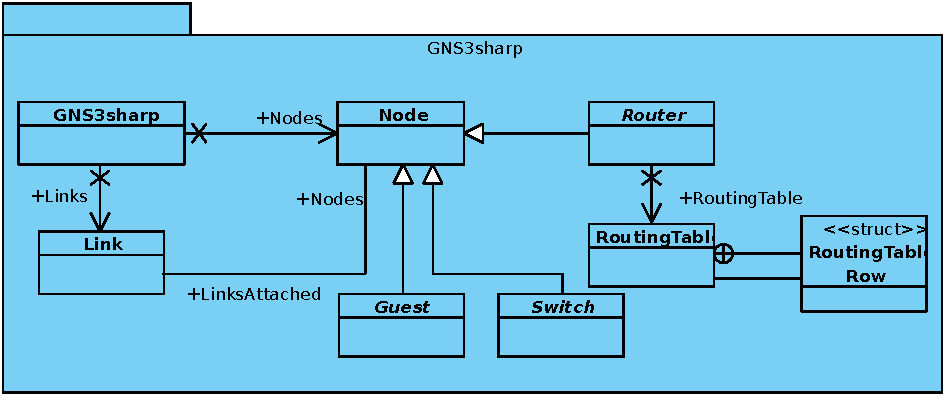
\includegraphics[scale=0.75]{imagenes/diagrama_api1}
  \caption{Boceto de diagrama UML de la API}
  \label{fig:diagrama_api1}
\end{figure}

A continuación pasamos a desarrollar cada una de las clases conceptualmente:

\subsubsection[''La clase principal'']{GNS3sharp, la clase principal}
Tal y como expusimos en la sección~\ref{subsec:accesoapi}, crearemos una clase principal que gestionará toda la interacción con el simulador de redes. Hemos llamado a esta clase del mismo modo que a la API, \GNSCS. Recalcamos entonces: los objetos que se encarguen de gestionar los proyectos serán del tipo \GNSCS.

¿Y en qué consistirá está gestión concretamente? Básicamente, esta clase debe encargarse de:
\begin{enumerate}
\item Establecer la conexión con el servidor de GNS3 y recopilar toda la información acerca del proyecto que se pretende controlar.
\item Convertir toda es información en objetos útiles que puedan ser utilizados.
\item Crear una gestión eficiente de esos recursos de manera que sean fácilmente accesibles y manipulables.
\end{enumerate}

Estos recursos de los que hablamos serán en gran medida los representados por las clases que se desarrollarán justo debajo.

Sin embargo, la creación de proyectos y despliegue de nodos en los mismos quedarán excluidos, ya sea por la complejidad añadida que conlleva o porque no son funciones que nos sean vitales para la construcción de juegos. Estas funcionalidades deberán ser llevadas a cabo manualmente. Más adelante podrán ser controladas desde la librería sin problema.

\subsubsection{Node}
Sin lugar a dudas es aquí donde se encuentra la característica más interesante de GNS3 y es hacia donde nuestros esfuerzos deben dirigirse. Dado que cada nodo representa un aparato de la red, lo ideal es que ese aparato pueda ser convertido a un objeto en nuestra biblioteca desde el que se nos permita su control. 

Esta es la finalidad de la clase \texttt{Nodo}. Su deber será el de contener todos los parámetros necesarios para habilitar la conexión con el nodo y así abrir un canal de comunicación con él; un canal que habilite tanto el envío como la recepción de mensajes.

Para la creación de las instancias de la clase se tendrá que recurrir a \GNSCS, que mediante los datos que recoja del servidor de GNS3 será capaz de crear asimismo el objeto.

Como GNS3 admite todo tipo de aparatos de red, cada uno con sus peculiaridades, lo más sensato es crear una clase para cada uno de esos equipos. Esta individualización permite definir métodos propios para cada elemento y, de este modo, facilitar su uso final. Tal y como se puede ver en el diagrama de la figura~\ref{fig:diagrama_api1}, definiremos tres clases principales (\texttt{Guest}, \texttt{Router} y \texttt{Switch}) que heredarán de \NODE. De estas clases nacerán asimismo otra serie de clases referidas a aparatos concretos y a no tipos genéricos.

\subsubsection{Link}
Los nodos están interconectados entre sí mediante enlaces. Representaremos cada uno de ellos mediante la clase \LINK. Esta clase guardará como objetos a los nodos que interconecta así como información sobre el propio enlace (cuánto jitter, latencia... posee). Al igual que \LINK, la generación de instancias de esta clase pasará por \GNSCS.

La clave de representar los enlaces en la API es que nos permitirá añadir, eliminar o incluso eliminarlos del proyecto desde el código, ampliando las posibilidades de interacción con el simulador.

\subsubsection{Otras clases}
Además de las anteriormente expuestas, se creará otra serie de clases que, o bien ayuden al desarrollo de la API (una clase con funciones de ayuda), o bien faciliten la representación de los datos (tal será el caso de \texttt{RoutingTable}, que puede atisbarse en la figura~\ref{fig:diagrama_api1}).

\subsection{GitHub y la comunidad}
Hemos considerado esencial que la API sea reutilizable. El objetivo de su desarrollo en ningún caso ha sido el de nacer y morir para el presente trabajo. Lejos de esto, se pretende que esta librería pueda ser utilizada por quien quiera, ya tenga como propósito la construcción de un videojuego o cualquier otra aplicación.

Con esto en mente, todo el código utilizado por la librería se encuentra disponible en \MYhref{https://github.com/aorestr/GNS3sharp}{este repositorio} de mi GitHub personal. Está liberado bajo una licencia MIT, tremendamente permisiva a la hora de reutilizar el código.

Además de los archivos de la propia API, se puede encontrar un README que explica algunos puntos importantes que considerar a la hora de utilizarla. En el repositorio de GitHub existe asimismo una sección de ``releases'', donde se suben los distintos compilados de la librería en formato ``.dll'' a medida que esta se expande o se reparan problemas aparecidos. Por supuesto, todo el código y su documentación están escritos en inglés para así llegar a más desarrolladores.

\section{Diseño del videojuego}
Establecida una plataforma sobre la que GNS3 pueda interactuar con código, llega el momento de diseñar el videojuego que haga uso de ella. 

\subsection{Interacción con el simulador}
A grandes rasgos, esto ya ha sido explicado. Ahora se va a dar una visión de la interacción desde el punto de vista del motor del videojuego; desde la creación del juego.

\begin{figure}[H]
  \centering
  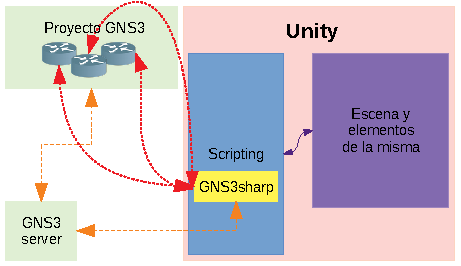
\includegraphics[scale=1.4]{imagenes/diagrama_interaccion}
  \caption{Diagrama de la interacción entre Unity y GNS3}
  \label{fig:diagrama_interaccion}
\end{figure}

Los proyectos de Unity están basados en un elemento llamado \GAOBJ. Todos los objetos que componen las escenas del proyecto se pueden abstraer en última instancia en ese tipo. El primer paso para que un proyecto de Unity pueda conectarse y controlar un esquema de red de GNS3 pasa por \textbf{insertar un \GAOBJ~ que tenga una instancia de la clase \GNSCS}. La única condición que se le impone a este objeto es que este parámetro contenido en él (la instancia) ha de ser accesible por todo el resto de elementos de la escena.

¿Para qué? Pura simplicidad: para que todos esos elementos no tengan que crear la suya propia. Creando una sola instancia de la clase centralizamos el trabajo en un solo objeto. La instancia contendrá información de los datos del proyecto de GNS3; información que podrá ser tomada por todos los componentes de la escena sin más que copiar la referencia al objeto. Si estos decidieran su propia instancia cada uno perdería en tiempo (la recopilación de datos desde el servidor no es instantánea) y en eficiencia.

La idea es que el jugador (en otros términos, el usuario final), posea interacción con el simulador de redes de forma que \textbf{las consecuencias puedan verse reflejadas en el juego}. Pongamos un ejemplo e invirtamos el orden lógico de desarrollo para entender mejor cómo funcionaría esto:

\begin{enumerate}
\item El jugador se encuentra en una habitación que no es más que una \textbf{representación de un router}. Tiene un botón justo delante suya. En la pantalla se le avisa de que si lo pulsa, la puerta asociada a una determinada interfaz se cerrará, de forma que los enemigos que se ven acercarse en esa dirección no podrán pasar. Lo pulsa entonces.
\item Ese botón es un \GAOBJ~ de la escena actual que tiene un \textit{trigger} asociado a él y un script que lo gestiona. Uno de los atributos de tal código es la referencia a la instancia del objeto \GNSCS, construido al arrancar la escena y que suponemos ya contiene toda la información del proyecto de GNS3. Cuando se activa el trigger (una condición del script pasa a ser \texttt{True}), se toma la referencia del objeto asociado al router donde el personaje está. Se utiliza tal objeto para enviar un comando al router que le haga apagar la interfaz correspondiente.
\item El mensaje llega al router. Este lo ejecuta y devuelve el resultado.
\item El script recibe la respuesta y, tras analizarla, confirma que la interfaz se ha cerrado. Envía un mensaje al \GAOBJ~ de la puerta para que la cierre.
\end{enumerate}

Este flujo es de alguna forma lo que se ha representado en la figura~\ref{fig:diagrama_interaccion}. El bloque morado hace referencia a todo el entorno que comprende una escena de Unity. Esta escena contendrá una serie de \GAOBJ s, cuyo comportamiento vendrá determinado mayormente mediante lógica programada por scripts. El bloque azul hace referencia a este compendio. Alguno de esos scripts será el encargado de contener una instancia de \GNSCS . Al ser creada, esta se conecta al servidor de GNS3 desde donde recibe toda la información del proyecto con el que se quiere trabajar. A partir de ahí, el resto de \GAOBJ s de la escena no tendrán más que usar esa instancia para poder conectarse a los nodos (entre otras cosas) de la simulación. 

\subsection{Modelo de videojuego}
Ahora que sabemos de qué forma se interconecta el juego con la red y en qué consiste exactamente la interacción, queda por concretizar qué clase de juegos podríamos crear. Hay que tener en mente en todo momento que pretendemos crear un \textbf{juego didáctico}, así que no nos vale cualquier construcción. La dificultad es, entonces, doble, pues es necesario seguir los cánones que dictan el buen hacer de un videojuego (véase un inteligente diseño de niveles, una estética atractiva y coherente, apartado técnico gráfico y sonoro propio, niveles a prueba de bugs...) a la vez que planear \textbf{qué} se quiere enseñar en ellos y \textbf{cómo} se pretende hacerlo.

Para sortear estas dificultades se ha decidido que la estructura del juego esté basada en pequeños niveles interconectados entre sí por una plataforma común. La linealidad de un juego exige de un guion y de una cohesividad de los que el juego ``federado'' puede permitirse  prescindir.

\begin{figure}[H]
  \centering
  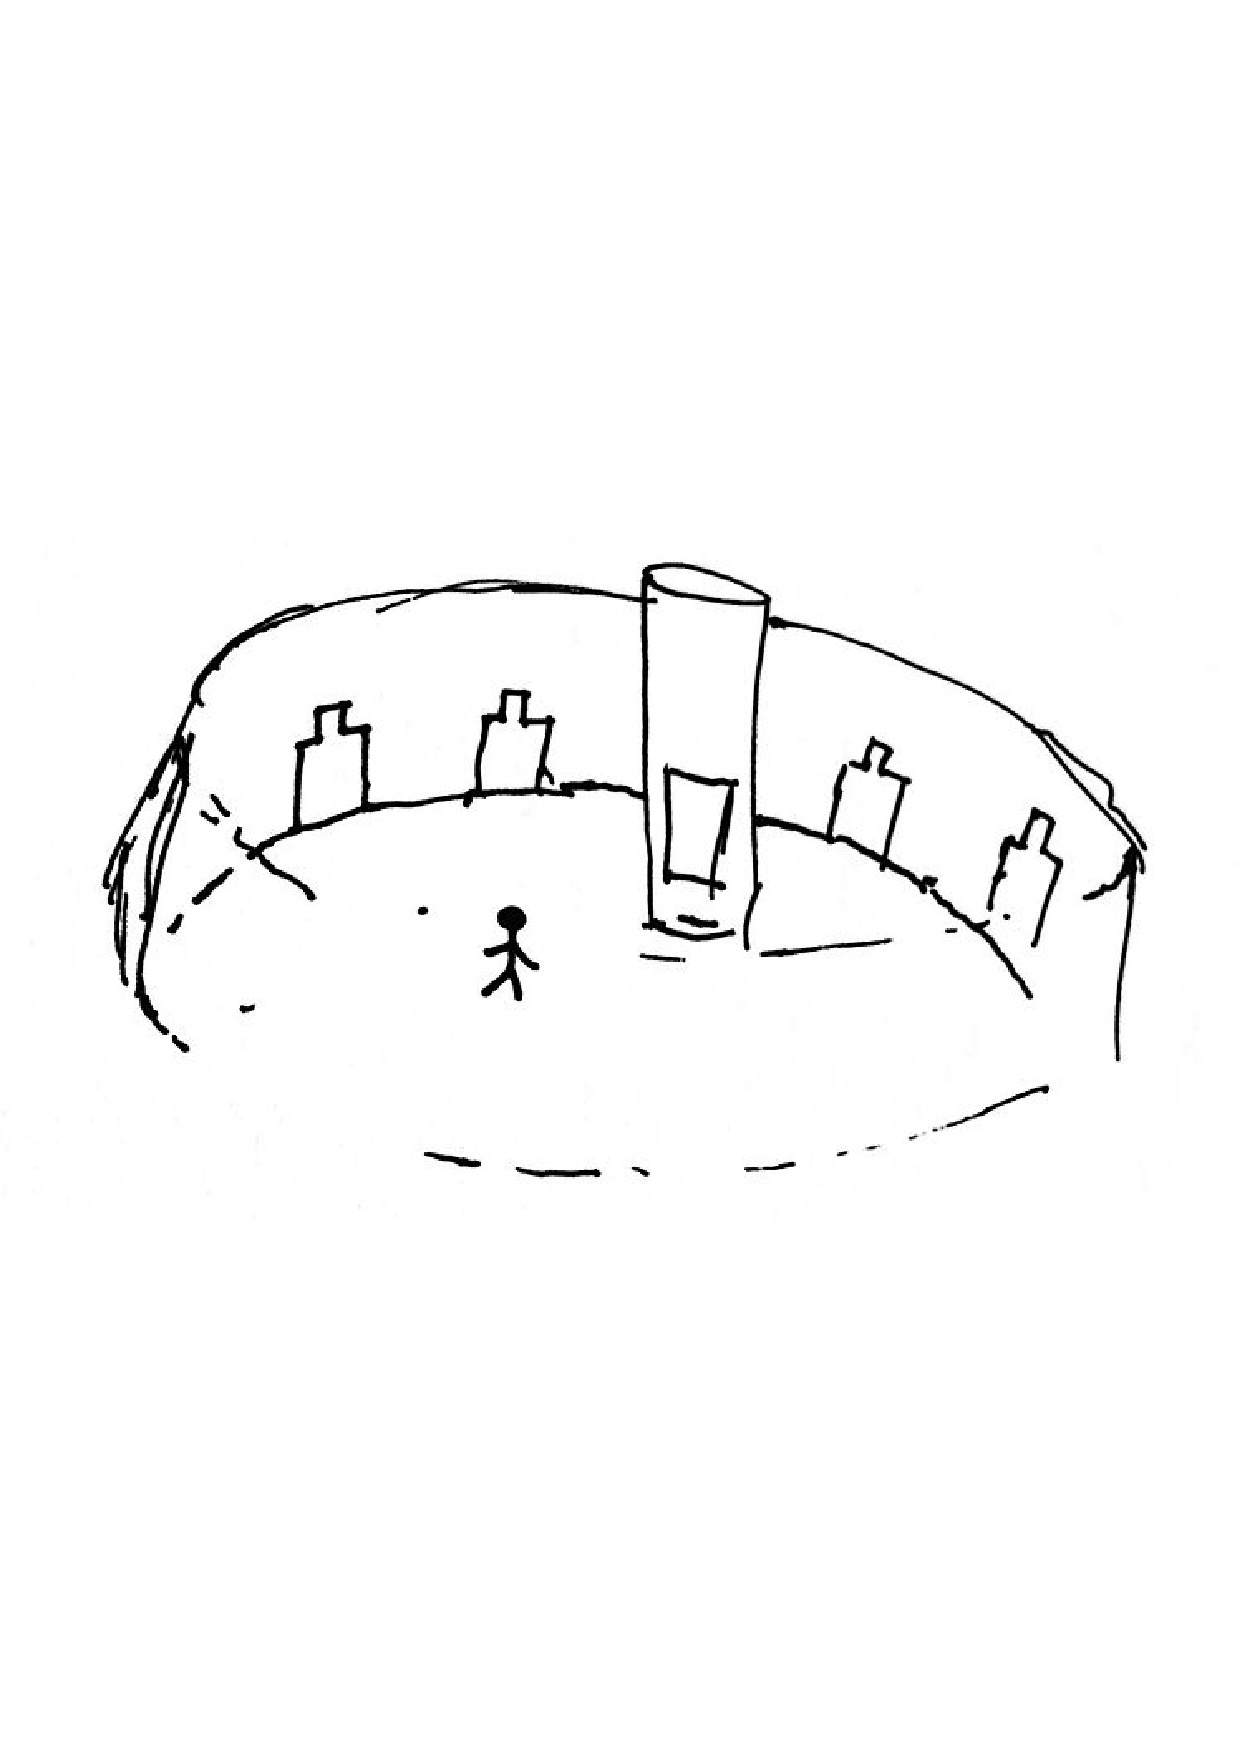
\includegraphics[scale=0.35, trim={0 9cm 0 9cm}]{imagenes/hall_juego}
  \caption{Boceto del juego}
  \label{fig:hall}
\end{figure}

En el boceto de la figura de arriba se quiere ejemplificar (de forma extremadamente simplista) en qué consistiría este diseño.
\begin{itemize}
\item Cada vez que el jugador entre en el juego se encontrará en una suerte de ``hall''. El hall estará acotado por paredes con un número determinado de puertas.
\item Estas puertas conducen a los distintos niveles del juego. Cada puerta corresponde a una lección diferente sobre redes y telemática. El jugador no tiene que superar una lección (un nivel, una zona) para acceder a la siguiente, sino que puede elegir qué quiere aprender indistintamente. Por supuesto, se podría vetar la entrada a una zona hasta que supere una concreta. Idealmente, cada nivel al que se accede contaría con varias fases que van incrementando en dificultad.
\item Al superar estas zonas, se desbloquea un ``manual'' acerca de lo aprendido en esa sala. Este manual puede ser consultado en un monitor localizado en el centro del hall. Gracias a esto, se podría repasar rápidamente lo aprendido en niveles anteriores desde un solo lugar.
\end{itemize}
Esta forma de acceder a los niveles es similar a la que siguen los videojuegos de la saga \textit{Crash Bandicoot} (\textit{2}, \textit{3}, \textit{La venganza de Cortex...}), donde existe una sala de ``descanso'' desde la que elegir cuál será la siguiente fase a jugar. Abstrayendo esta idea algo más, no es más que un menú estático desde donde elegir el nivel (juegos de corte más ``clásico'' como \textit{Super Meat Boy} utilizan este patrón) salvo que gozando de una interacción más directa y natural con el jugador, integrándolo más.

Existen dos aproximaciones al modo en el que estos niveles se conectan con el simulador de redes:
\begin{itemize}
\item Por un lado, podría existir \textbf{un proyecto de GNS3 por cada nivel} y/o fase. Aunque mucho más estructurado y por ende posiblemente más sencillo de gestionar, es necesario establecer conexión con el servidor de GNS3 por cada nivel para recopilar la información del mismo. Esto se traduce en tiempo. Además, el servidor de GNS3 no registra el proyecto de GNS3 a menos que este se abra manualmente desde GNS3 en una sesión. Más tiempo.
\item La otra solución pasa por crear \textbf{un solo proyecto} para todo el juego. Sería necesario desplegar todos los aparatos que vayan a ser utilizados en él, incrementando altamente los recursos que el sistema utiliza. Para paliar este último problema existen dos opciones:
\begin{enumerate}
\item Encender los aparatos que vayan a ser necesitados en el nivel a jugar y cerciorarse de que el resto permanece apagado.
\item Reconfigurar los aparatos que vayan a ser utilizados para que sus propiedades se correspondan a lo que se necesita para el respectivo nivel.
\end{enumerate}
De entre estos dos acercamientos al problema, quizás el primero sea más simple, pero el arranque de cada nodo no es inmmediato. El segundo entraña una mayor dificultad ingenieril y mayor propensión al error aunque la configuración de los aparatos conlleve menos tiempo.
\end{itemize}

Sin embargo, aunque todas estas ideas pueden sonar realmente interesantes, el juego final desarrollado no ha podido alcanzarlas. En el siguiente capítulo, donde se detalla la integración real de lo expuesto en este capítulo, se comprobarán cuáles han sido las dificultas encontradas en el camino que han frenado de una forma u otra el prometedor escenario inicial. 
%
%\chapter{Implementación}\label{chap:Integration}
Trazado el esquema del trabajo a realizar, el siguiente paso es lógicamente llevarlo a cabo. Las soluciones empleadas para todo el proceso será lo que compongan este capítulo.

\section{Desarrollo de la API}
Si bien en la sección~\ref{sec:dis_api} ya se habló de la estructura con la que nuestra API contaría, en esta ocasión se contará con todo detalle el modo en el que esta ha sido desarrollada. Se describirán los puntos más importantes de cada una de las clases así como el modo en que fueron originados. Naturalmente, no se pretende explicar todo el contenido, pues no es su propósito. Se evitará así explicar en muchos casos métodos y propiedades privadas para centrarnos en aquellas públicas.

Para finalizar se explicará la relación existente entre las clases con ayuda de un diagrama UML así como la forma en la que estas han sido compiladas para ser unificadas como librería.

Todas estas clases conforman un único \texttt{namespace} o espacio de nombres. Conviene recalcar que la API ha sido enteramente desarrollada desde cero.

\subsection[GNS3sharp]{\href{https://github.com/aorestr/GNS3sharp/blob/master/gsn3sharp.cs}{GNS3sharp}}\label{subsec:gnscsclass}
\subsubsection{Constructor}
El constructor de \GNSCS~es sin duda uno de los elementos más importantes de toda a API. ¿Por qué? Tendrá la responsabilidad de conectarse al servidor de GNS3, recibir todos los datos de un cierto proyecto que solicitemos, procesarlos y guardarlos de tal forma que sean útiles. Su cabecera se muestra justo a continuación:
\begin{lstlisting}[language={[Sharp]C}, caption={Cabecera del constructor de \texttt{GNS3sharp}}, label={gnscs1}]
public GNS3sharp(string _projectID, string _host = "localhost", ushort _port = 3080)
\end{lstlisting}

Cosas que serán necesarias entonces para inicializarlo:
\begin{itemize}
\item \textbf{ID del proyecto}: cada proyecto de GNS3 tiene un ID asociado que el servidor guarda junto a su referencia. Más adelante, en la subsección \ref{subsec:aux}, veremos cómo no es necesario conocer el ID del proyecto sino que con el nombre del mismo será más que suficiente.
\item \textbf{Host}: la dirección del equipo donde el servidor está alojado. Por defecto se toma \texttt{localhost}; se supone que la mayor parte de las veces se encontrará en el mismo equipo desde el que se utiliza la API.
\item \textbf{Puerto}: además de la dirección del servidor, es necesario conocer el puerto en el que está montado. GNS3 determina el \texttt{3080} por defecto.
\end{itemize}

De acuerdo, ¿y qué hace exactamente con estos tres parámetros?
\begin{enumerate}
\item Crea la cadena de texto de la URI donde está el recurso asociado a los nodos del proyecto. En esta dirección existe únicamente un JSON con toda la información sobre él. Se instancia un cliente web y \textbf{se descarga el recurso como cadena de texto}.

\item Hay que \textbf{deserializar el JSON}. Este paso no es en absoluto trivial, ya que los métodos de \textit{Json.NET} son incapaces de extraer los datos que necesitamos directamente. Así que, valiéndonos de las herramientas en forma de clases que nos ofrece, lo hacemos manualmente.
\begin{lstlisting}[language={[Sharp]C}, caption={Deserialización de JSON}, label={gnscs2}]
// JSON array object
JArray jsonArray = JArray.Parse(json);
Dictionary<string,object> tempDict = new Dictionary<string, object>();

// Variables in which store the JSON info temporaly
string name; object value;        
if (jsonArray.HasValues){
    foreach (JObject jO in jsonArray.Children<JObject>()) {
        foreach (JProperty jP in jO.Properties()) {                
            name = jP.Name;
            value = (object)jP.Value;
            tempDict.Add(name,value);
            // The last key of every node
            if (jP.Name.Equals(lastKey)) {
                // If we do not copy the content of the dictionary into another
                // we will be copying by reference and erase the content once
                // we 'clear' the dict
                Dictionary<string, object> copyDict = new Dictionary<string, object>(tempDict);
                dictList.Add(copyDict);
                tempDict.Clear();
            }
        }
    }
}
\end{lstlisting}
Sin entrar mucho al detalle, lo que hace es parsear el objeto como objeto de tipo \texttt{JArray} y luego este se discretiza por cada elemento de esa cadena. Cada elemento representa a un nodo. Se recorre a su vez cada subelemento que lo conforma, que no son más que sus pares \textit{llave-valor}.

Los datos que se han extraído se guardan en una lista de diccionarios de par \texttt{<string,object>}. Se usa la clase genérica \texttt{object} porque el tipo del valor asociado a la clave varía.

\item Se hace lo mismo para los enlaces. El proceso es similar.

\item A partir de los objectos extraídos de la deserialización del JSON, se \textbf{crean las instancias representantes} de los nodos del proyecto. Existe un problema de cierta gravedad en esto: en el JSON no existe ningún parámetro que explicite de que tipo de nodo estamos hablando. Es decir, que no podemos conocer directamente con qué aparato concreto estamos tratando.

La solución que nosotros hemos tomado para sortear este problema es el añadir una etiqueta al nombre del nodo en el momento de la creación de la red en GNS3. Por ejemplo, si el nodo es un \textit{VPC} (nodo predefinido y propio del simulador), su nombre sería de la forma ``[VPC]NombreDelNodo''. Será necesario entonces definir una etiqueta por cada tipo de aparato a utilizar.

Sin embargo, sigue existiendo un problema de peso en todo esto: no conocemos el tipo de cada nodo antes del tiempo de ejecución (\textit{runtime}, en inglés) del código. En otras palabras, hasta el momento de la descarga y el análisis del JSON es imposible saber con qué tipo de nodos estamos lidiando, con lo que es a su vez imposible escribir el constructor que se va a utilizar. Recordemos que nuestra intención es usar una clase por cada modelo de nodo concreto. Por supuesto, se podría crear una sentencia condicional en la que, dependiendo de la etiqueta, llevara al constructor de una clase u otra. Sin embargo, requeriría de muchas líneas de código y sería necesario añadir más cada vez que se introduzca una nueva clase de modelo de aparato en la API.

La solución pasa entonces por lo que en programación se conoce como \textit{reflexión}. Poniéndolo en términos puramente técnicos: ``inspeccionar los metadatos y el código compilado en tiempo de ejecución se llama reflexión''\cite{csnutshell}.

\begin{lstlisting}[language={[Sharp]C}, caption={Instanciación de los nodos}, label={gnscs3}]
System.Reflection.ConstructorInfo ctor; int i = 0;
try{
    foreach(Dictionary<string, object> node in JSON){
        try{
            Console.WriteLine($"Gathering information for node #{i}... ");

            // Get the main constructor of the node type
            ctor = Aux.NodeType(node["name"].ToString()).GetConstructors(
                System.Reflection.BindingFlags.NonPublic | System.Reflection.BindingFlags.Instance
            ).Last();

            // Invoke the previous constructor and create the instance through it
            listOfNodes[i] = (Node)ctor.Invoke(
                new object[]{
                    node["console_host"].ToString(), 
                    ushort.Parse(node["console"].ToString()), 
                    node["name"].ToString(),
                    node["node_id"].ToString(),
                    GetNodeListOfPorts(node)
                }
            );
            
            nodesByName.Add(listOfNodes[i].Name, listOfNodes[i]);
            nodesByID.Add(listOfNodes[i].ID, listOfNodes[i]);
        } catch(Exception err1){
            Console.Error.WriteLine(
                "Impossible to save the configuration for the node #{0}: {1}", 
                i.ToString(), err1.Message
            );
        }
        i++;
    }
} catch(Exception err2){
    Console.Error.WriteLine(
        "Some problem occured while saving the nodes information: {0}",
        err2.Message
    );
    listOfNodes = null;
}
\end{lstlisting}
Con esto en mente pues, tomamos el tipo de la clase asociada al aparato mediante la etiqueta que ya hemos mencionado. Obtenemos gracias a él el constructor que nos es útil. El siguiente paso es invocarlo para generar la instancia del objeto. Previamente se pensó en utilizar el método \texttt{Activator.CreateInstance()}, que instancia un objeto directamente con los metadatos del tipo representante (representados a su vez por la clase \texttt{System.Type}) y los parámetros del constructor, pero solo funciona cuando los constructores son públicos y no es el caso de aquellos que usamos.

Añadimos la instancia a una lista donde se guardan todos los objetos representantes de los nodos. Esta propiedad se verá más adelante.

La obtención de las interfaces que cada nodo posee así como de cuáles están libres y cuáles están usadas por cierto enlace requiere de más trabajo que no se considera necesario explicar aquí.

\item Es ahora el momento de instanciar los enlaces a través de la información extraída previamente. Aunque el problema que vimos con los nodos no se va a dar aquí, la obtención de los enlaces y sus parámetros tampoco es fácil. La principal dificultad aparece, una vez más, cuando se trata con las interfaces de los nodos.

\begin{lstlisting}[language={[Sharp]C}, caption={Matcheo entre los enlaces y las interfaces de los nodos}, label={gnscs4}]
List<Dictionary<string,object>> dictList = null;
try{
    dictList = DeserializeJSONList(nodesJSON, "port_number");
} catch (Exception err){
    Console.Error.WriteLine(
        "Some problem occured while trying to gather information about the nodes connect to the link: {0}",
        err.Message
    );
}

if (dictList.Count > 0){
    // Iterates through the JSON dictionary
    foreach (Dictionary<string, object> nodeTemp in dictList){
        // Iterates through the nodes the link connects
        foreach (Node node in link.Nodes){
            if (node != null && node.ID.Equals(nodeTemp["node_id"].ToString())){
                // Search for the port that matches the found one
                var foundPort = node.Ports.Where(
                    x => (
                        x["adapterNumber"].ToString() == nodeTemp["adapter_number"].ToString() &&
                        x["portNumber"].ToString() == nodeTemp["port_number"].ToString()
                    )
                );
                // If exists, add the link into the key "link" of the ports list
                // of dictionaries of the node
                if (foundPort.Count() > 0) foundPort.First()["link"] = link;
            }
        }
    }
}
\end{lstlisting}

Una vez localizada la sección relacionada con los nodos en el diccionario que contiene la información de los enlaces extraída del JSON, se deserializa y se hace un barrido por entre esos nodos. Hecho esto, se busca entre los nodos que ya tenemos almacenados aquel que posea la misma ID que el del nodo sobre el que estamos barriendo. Si se encuentra, se busca la interfaz del mismo que dicte el nodo del barrido. De encontrarse, el puerto (usado aquí como sinónimo de interfaz) del nodo que teníamos almacenado guardará la información del enlace que contiene todos esos nodos que se están analizando. Es bastante confuso, sí.

El método principal que se encarga de la extracción de los enlaces, \texttt{GetLinks()}, se verá ayudado por un par de funciones declaradas localmente. Estas funciones locales aparecen por vez primera en C\#7.

Se guardan todos estos enlaces como lista en otra de las propiedades que se verán más adelante.

\item Finalmente, se añade a cada nodo la información de los enlaces a los que está conectado.

\end{enumerate}

\subsubsection{Propiedades}
\begin{itemize}
\item \texttt{ProjectID}, \texttt{Host} y \texttt{Port}: propiedades que se toman directamente de los parámetros que el constructor necesitaba.
\item \texttt{NodesJSON} y \texttt{LinksJSON}: diccionarios que contienen los JSON descargados desde el servidor una vez han sido parseados. Por lo general esta propiedad no tendría porque ser usada por un usuario que no esté desarrollando la API, pero se mantiene como \texttt{public} por si hay algún caso en el que sí.
\item \texttt{Nodes} y \texttt{Links}: posiblemente las propiedades más importantes de la clase. Son listas que contienen los objetos que representan los nodos y enlaces, respectivamente, del proyecto.
\end{itemize}

\subsubsection{Métodos}
La mayor parte de los métodos de esta clase son privados, pues son usados internamente como subrutinas de otros métodos más grandes. Sin embargo podemos encontrar algunos accesibles desde fuera de la clase:
\begin{itemize}
\item \texttt{StartNode()} y \texttt{StopNode()}: activan/desactivan un nodo del proyecto. Esto se consigue haciendo uso del método POST de REST hacia la URI correspondiente al nodo. En el código se lleva a cabo mediante la clase \texttt{System.Net.Http.HttpClient}, que provee las herramientas suficientes para enviar y recibir datos de un recurso web.

\begin{lstlisting}[language={[Sharp]C}, caption={Activación/desactivación de un nodo}, label={gnscs5}]
// First part of the URL
string URLHeader = $"http://{host}:{port}/v2/projects/{projectID}/nodes";

// Pack the content we will send
ByteArrayContent byteContent = null;
try{
    string content = JsonConvert.SerializeObject(new Dictionary<string, string> { { "", "" } });
    byteContent = new ByteArrayContent(System.Text.Encoding.UTF8.GetBytes(content));
    byteContent.Headers.ContentType = new MediaTypeHeaderValue("application/json");
} catch(JsonSerializationException err){
    Console.Error.WriteLine("Impossible to serialize the JSON to send it to the API: {0}", err.Message);
}

if (byteContent != null){
    try{
        responseStatus = HTTPclient.PostAsync(
            $"{URLHeader}/{node.ID}/{status}", byteContent
        ).Result.IsSuccessStatusCode;
    } catch(HttpRequestException err){
        Console.Error.WriteLine("Some problem occured with the HTTP connection: {0}", err.Message);
        responseStatus = false;
    } catch(Exception err){
        Console.Error.WriteLine("Impossible to {2} node {0}: {1}", node.Name, err.Message, status);
        responseStatus = false;
    }
} else{
    responseStatus = false;
}
\end{lstlisting}

\item \texttt{StartProject()} y \texttt{StopProject()}: activan/desactivan todos los nodos del proyecto. Se intentó paralelizar el activado/desactivado de los nodos sin resultado.
\item \texttt{SetLink()}: pasándole los objetos representantes de dos nodos del proyecto, es capaz de descubrir cuáles de sus interfaces están vacías y, de haber, crea un enlace entre ellas. También se consigue mediante POST. Actualiza \texttt{Links} y otra serie de parámetros tras la inserción. Es un método de cierta longitud (algo más de 100 líneas sin contar otras definidas fuera de las que hace uso). En este método y en similares es muy recurrido el tipo \texttt{dynamic}, que obliga al compilador a averiguar el tipo real de la variable en el momento de ejecución del código. Algo similar a lo que ocurre en lenguajes interpretados como Python y Matlab.
\item \texttt{EditLink()}: método polimórfico, pues dependiendo de si su parámetro es un \LINK~o dos \NODE~su comportamiento varía. Se parece a \texttt{SetLink()} pero este hace PUT y no POST a la URI. Ambas formas del método llaman a un método interno de \LINK. Tal y como su nombre indica, edita un enlace, permitiendo hacer variar los parámetros del mismo.
\item \texttt{RemoveLink()}: con la misma base polimórfica que el anterior. Elimina un enlace del proyecto de GNS3 con un DELETE e inmediatamente a su representante objeto.
\item \texttt{GetNodeByName()} y \texttt{GetNodeByID()}: dado un nombre o un identificador, respectivamente, devuelve el objecto representante de tal nodo.
\end{itemize}

\subsection[Node]{\href{https://github.com/aorestr/GNS3sharp/blob/master/node.cs}{Node}}
\subsubsection{Constructor}
El constructor principal de \NODE~solo es llamado desde \GNSCS. Es bastante sencillo: asigna parámetros básicos que la instancia de \GNSCS~toma del servidor. Entre ellos se encuentra la dirección del nodo. Gracias a ella y mediante otro método interno de la clase, se crea un cliente TCP y se establece un flujo de conexión para el envío y recepción de mensajes.

\begin{lstlisting}[language={[Sharp]C}, caption={Establecimiento de la conexión con el nodo}, label={node2}]
protected (TcpClient Connection, NetworkStream Stream) Connect(int timeout = 10000){
    // Network endpoint as an IP address and a port number
    IPEndPoint address = new IPEndPoint(IPAddress.Parse(this.consoleHost),this.port);
    // Set the socket for the connection
    TcpClient newConnection = new TcpClient();
    // Stream used to send and receive data
    NetworkStream newStream = null;
    try{
        newConnection.Connect(address);
        newStream = newConnection.GetStream();
        newStream.ReadTimeout = timeout; newStream.WriteTimeout = timeout;
    } catch(Exception err){
        Console.Error.WriteLine("Impossible to connect to the node {0}: {1}", this.name, err.Message);
        newConnection = null;
    }
    return (newConnection, newStream);
}
\end{lstlisting}

Especial atención a este método, que devuelve una tupla (recordemos, también nuevo en C\#7) en lugar de una simple variable.

Para que solo clases que pertenecen a esta librería puedan hacer uso del constructor, se ha aplicado el modificador de clase \texttt{internal}, el cual solo permite llamadas desde el espacio de nombres donde esté definido. Encapsulamiento en estado puro. La API no permite la creación de nodos nuevos así que se ha optado por ocultar este método del desarrollador final.

No obstante, sí que se incluye un constructor-clonador. Se trata de un constructor de clase cuyo parámetro de entrada es otro \NODE, de forma que se replica enteramente en una nueva instancia.

\begin{lstlisting}[language={[Sharp]C}, caption={Clonador de nodos}, label={node2}]
public Node(Node clone){
    this.consoleHost = clone.ConsoleHost; this.port = clone.Port;
    this.name = clone.Name; this.id = clone.ID; this.ports = clone.Ports;
    this.tcpConnection = clone.TCPConnection; this.netStream = clone.NetStream;
}
\end{lstlisting}

\subsubsection{Propiedades}
\begin{itemize}
\item \texttt{ConsoleHost} y \texttt{Port}: dirección y puerto donde el nodo está ubicado. Gracias a estos datos podremos establecer una conexión con el aparato.
\item \texttt{Name} y \texttt{ID}: nombre e identificador único del nodo. El nombre debería comenzar por \textit{[$<$EtiquetaDelNodo$>$]} para que \GNSCS~sea capaz de construir el objeto con la clase asociada a tal aparato.
\item \texttt{Ports}: interfaces que posee el nodo. Es un diccionario de tres llaves: ``adapterNumber'', ``portNumber'' y ``link''. Los dos primeros son parámetros que GNS3 asigna a las interfaces. El último guarda la referencia del enlace asociado a la interfaz en caso de que esté siendo utilizada y \texttt{null} si no.
\item \texttt{LinksAttached}: lista de \LINK. Referencias a los que el nodo está conectado.
\end{itemize}

\subsubsection{Métodos}
Esta clase destaca por sus dos métodos principales: \texttt{Send()} y \texttt{Receive()}.

\begin{itemize}
\item \texttt{Send()}: haciendo uso del flujo establecido durante la creación del objeto, se envía una cadena de texto previamente convertida a bytes. Antes de enviar cualquier mensaje, comprueba que es posible escribir en el canal.

\begin{lstlisting}[language={[Sharp]C}, caption={Envío de mensajes a un nodo}, label={node3}]
byte[] out_txt = Encoding.Default.GetBytes($"{message}\n");
this.netStream.Write(buffer: out_txt, offset: 0, size: out_txt.Length);
this.netStream.Flush();
\end{lstlisting}

\item \texttt{Receive()}: algo más complejo que \texttt{Send()}, hace también uso del canal establecido, aunque necesita de pasos adicionales para gestionar correctamente la información que se recibe.

Cada mensaje recibido se convierte en una cadena de texto que va siendo añadida a una lista. A cada nueva recepción se consulta al canal si existe nueva información a leer; si no, se esperan unos segundos confiando en que existan datos a procesar por parte del servidor. Se vuelve a hacer la comprobación y, si efectivamente no queda nada más por leer, se analizan las líneas recibidas en busca de caracteres inválidos y se guardan. 

\end{itemize}

\subsubsection{Destructor}
Esta es la única clase de la librería que hace uso de un destructor personalizado. Los destructores ayudan a definir las sentencias que serán ejecutadas junto antes de que el objeto en cuestión sea destruido (se desreferencie).

Únicamente se encarga de cerrar la conexión establecida con el nodo.

\subsection{Herederos de Node}
La clase \NODE~no hace más que de padre para todo un abanico de clases. A partir de ahí se crea una estructura en árbol desde la que se ramifica una serie de subclases. Las tres herederas directas son \texttt{Router}, \texttt{Switch} y \texttt{Guest}, correspondientes a los tres amplios grupos de nodos que pueden encontrarse en GNS3. Estas tres clases son abstractas; su labor no es otra que la de declarar métodos importantes que cada uno de estos aparatos se espera que posean.

La definición de los métodos se encuentra en sus clases herederas, que no representan otra cosa que dispositivos concretos. Pongamos un ejemplo para que se vea más sencillo:

\NODE~es la clase padre. Define el constructor, la forma de establecer la conexión con los nodos y los métodos para enviar y recibir mensajes de estos. De esta clase parte otra, \texttt{Router}, que por consiguiente es hija suya. Esta clase declara métodos abstractos que se espera que las clases representantes de los routers posean, como por ejemplo \texttt{GetIPByInterface()}, que dado el nombre de una interfaz ha de ser capaz de averiguar cuál es su IPv4 asociada. Finalmente, la clase \texttt{OpenWRT} va a heredar de \texttt{Router}. Definirá los métodos abstractos de la anterior y los suyos propios.

Es muy importante señalar que cada una de estas clases representantes de aparatos concretos deberán contar con una propiedad estática que contiene la etiqueta que el nodo deberá tener en su nombre. De nuevo con ejemplo: si queremos que el constructor de \GNSCS~pueda construir correctamente el objeto representante a un router OpenWRT de nuestro proyecto de GNS3, es necesario que a este se le ponga por nombre algo como \textit{[OPENWRT]NombreDelRouter}. De esta forma, automáticamente y una vez más haciendo uso de reflexión, la API es capaz de encontrar la clase a la que se hace referencia.

\begin{lstlisting}[language={[Sharp]C}, caption={Etiqueta de \texttt{OpenWRT}}, label={herederosnode1}]
private const string label = "OPENWRT";
/// <summary>
/// Label you must set in the name of the node at the GNS3 project
/// <para>Name of the node must look like "[OPENWRT]Name"</para>
/// </summary>
/// <value>Label as a string</value>
public static string Label { get => label; }
\end{lstlisting}

Si se hace correctamente, se instanciará un objeto \texttt{OpenWRT}. De lo contrario, se optará por el genérico \NODE.

Este punto del trabajo es importante. Una de las cosas que más nos interesaban de la creación de la API era su reutilización por manos ajenas. La estructura establecida en ella permite que cualquiera que quiera hacer uso de ella y pretenda implementar un cierto tipo de nodos en su proyecto de GNS3 lo tenga fácil a la hora de crear un tipo que le dé soporte en la librería.

Actualmente GNS3 cuenta con implementaciones de docenas de dispositivos de gestión de red del mercado. Crear una clase representante de todas ellas es ciertamente un trabajo inviable. Sin embargo, se ha buscado que cada usuario que haga uso de ella lo tenga fácil para insertar la que necesite. Tan solo necesita añadir una clase que herede de su tipo de aparato correspondiente (\texttt{Router}...) y definir los métodos que le gustaría que esta tuviera.

El número de métodos definidos para cada clase va en función de las necesidades de cada uno. Un dispositivo real cuenta con cientos de funciones; abstraerlas todas como métodos es descabellado.

A continuación se muestra uno de los métodos que nosotros hemos generado para \texttt{OpenWRT}, clase que ha sido usada abundantemente en la integración final de este proyecto ya que el router al que hace referencia nos ha sido de gran utilidad.

\begin{lstlisting}[language={[Sharp]C}, caption={Método \texttt{GetIPByInterface()} de \texttt{OpenWRT}}, label={herederosnode2}]
public override string[] GetIPByInterface(string iface){

    string GetParameterIfconfig(string _iface, string type){

        string result = null; string command = null;
        if (type.Equals("IP"))
            command = $"ifconfig {_iface} | grep 'inet addr' | cut -d: -f2 | awk '{{print $1}}'";
        else if (type.Equals("NETMASK"))
            command = $"ifconfig {_iface} | grep 'inet addr' | cut -d: -f4 | awk '{{print $1}}'";
        if (command != null){
            string lineTemp;
            Send(command);
            foreach (string line in Receive()) {
                lineTemp = line.Trim();
                if (Aux.IsIP(lineTemp)){
                    result = lineTemp;
                    break;
                }
            }
        }
        return result;

    }

    return new string[]{ 
        GetParameterIfconfig(iface, "IP"), GetParameterIfconfig(iface, "NETMASK") 
    };
    
}
\end{lstlisting}

El método se encarga de encontrar la IP relacionada con cierta interfaz del router. Básicamente, envía un comando al router mediante \texttt{Send()} y de la respuesta obtenida con \texttt{Receive()} extrae la IP.

La conclusión que ha de sacarse de esto es que todos los métodos, o la mayor parte de ellos, van a ser definidos en base a estas dos funciones, \texttt{Send()} y \texttt{Receive()}. Podemos llevar esta lógica algo más allá: si no existe método creado en cierta clase para realizar una operación que nos es necesaria, podemos hacer uso de aquellas dos funciones para, sobre la marcha, conseguir lo que esperamos.

\subsection[Link]{\href{https://github.com/aorestr/GNS3sharp/blob/master/link.cs}{Link}}
\subsubsection{Constructor}
Una vez más, el constructor es únicamente accesible desde el espacio de nombres y solo será llamado desde \GNSCS. Se han definido dos concretamente: uno que supone que todos los parámetros del enlace de GNS3 son nulos (es un enlace ideal) y otro que supone que al menos uno de ellos es distinto.

\subsubsection{Propiedades}
\begin{itemize}
\item \texttt{ID}: identificador único del nodo. Como el resto de IDs, lo asigna automáticamente GNS3.
\item \texttt{Nodes}: array de objetos \NODE~que contienen los objetos representantes de los nodos que el enlace une en el proyecto.
\item Parámetros del enlace: \texttt{FrequencyDrop}, \texttt{PacketLoss}, \texttt{Latency}, \texttt{Jitter} y \texttt{Corrupt}. Son parámetros que GNS3 permite para eliminar idealidades de las conexiones. Todos son números enteros.
\end{itemize}

\subsubsection{Métodos}
Esta clase solo cuenta con un método, \texttt{EditLink()}. Permite editar uno de los parámetros del enlace. Para ello, además de ser este alterado en el objeto, se modifica en el proyecto de GNS3 haciendo un PUT a la URI asociada al enlace. Ya se mencionó este método tratando uno de los de \GNSCS.

\subsection{Clases auxiliares}\label{subsec:aux}
\begin{itemize}
\item \texttt{Aux}: define métodos de ayuda para otras clases del espacio de nombres como un identificador de direcciones IP. También se encarga de generar, mediante reflexión, un mapeo entre los tipos de nodos existentes en la API y la etiqueta asociada a ellos. Todo esto es realizado de forma automática.
\item \texttt{RoutingTable}: define una estructura para las tablas de enrutamiento. Es usada por las clases herederas de \texttt{Router} para una gestión más eficiente de esas tablas. Dentro de la propia clase se define un \texttt{struct} usado para trabajar más cómodamente con cada una de las rutas de la tabla. 
\item \texttt{ServerProjects}: en esta clase deben definirse métodos asociados a la URI del server donde se lista el conjunto de proyectos definidos en él. Por el momento solo cuenta con un método (\texttt{GetProjectIDByName()}) que extrae el ID de un proyecto dado su nombre, realmente útil a la hora de instanciar \GNSCS.
\end{itemize}

\subsection{Estructura de la API}
A continuación se muestra el diagrama UML de la API, desde el que puede observarse esquemáticamente el diseño de cada una de las clases y la relación que existe entre ellas.

\begin{figure}[h]
  \centering
  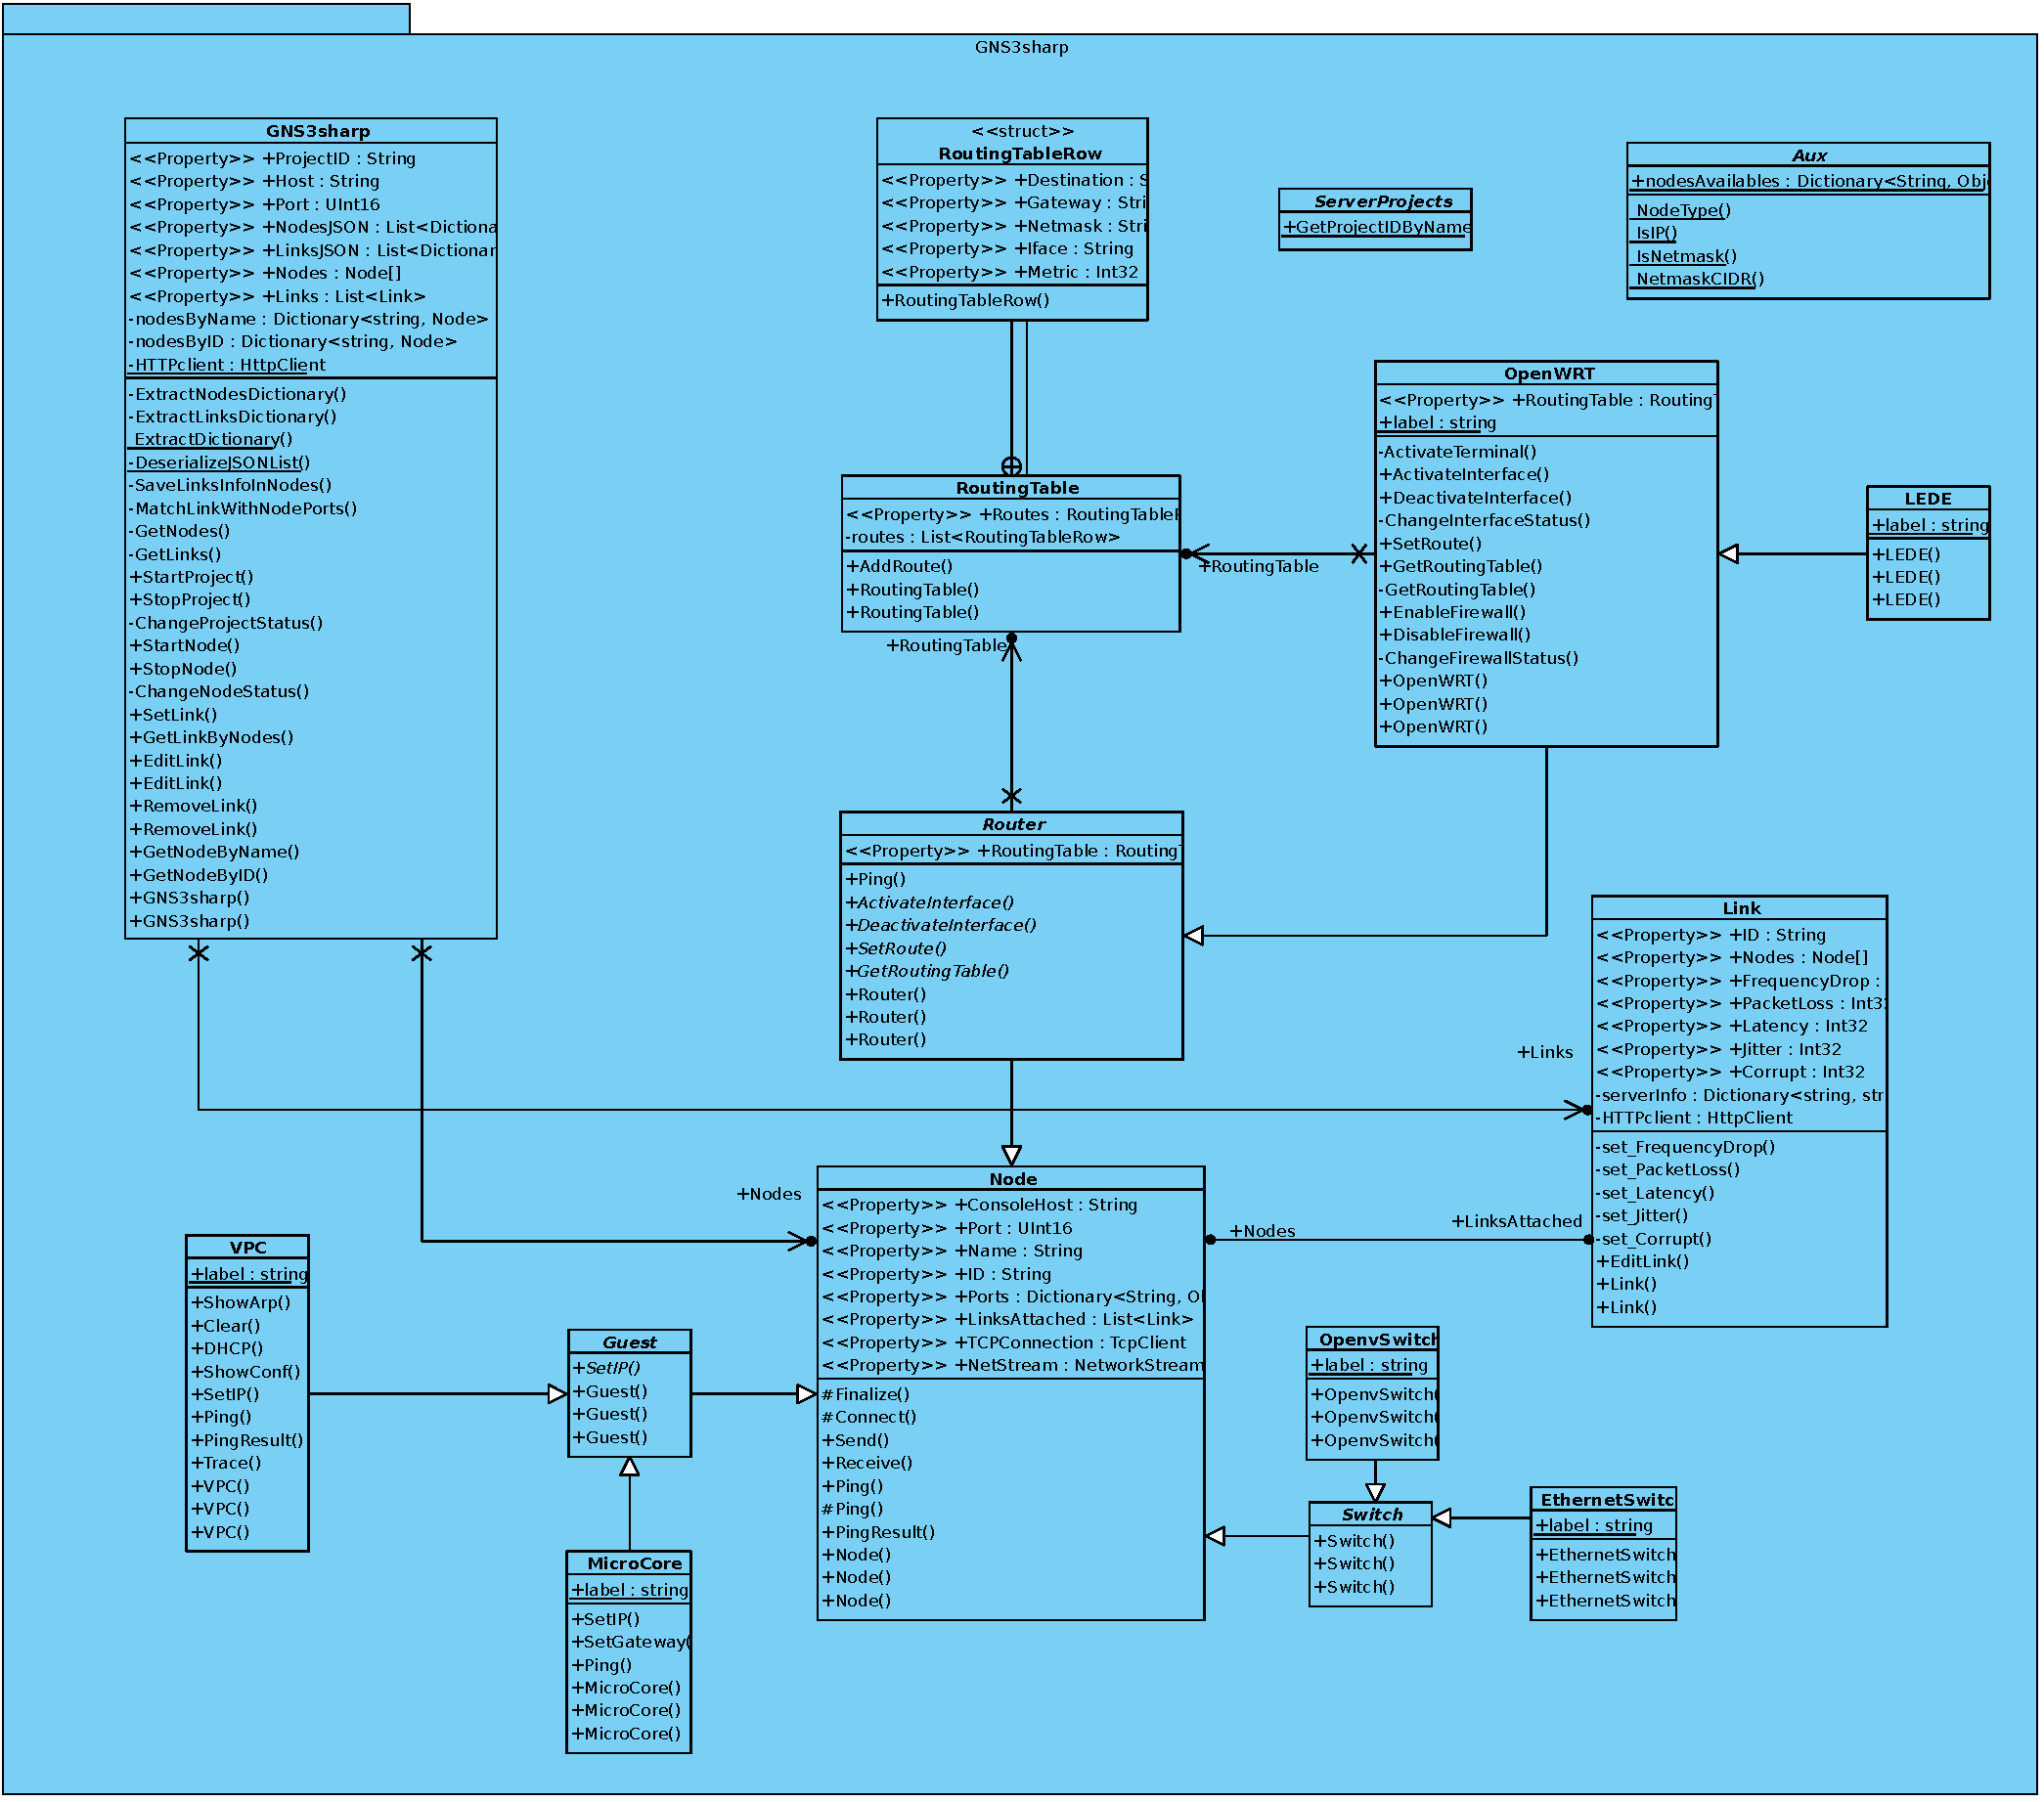
\includegraphics[scale=0.4]{imagenes/diagrama_api2}
  \caption{Diagrama UML de la API}
  \label{fig:uml_api}
\end{figure}

\subsection{Compilación} \label{subsec:compilation}
C\# es un ``lenguaje gestionado'' (del inglés \textit{managed code}) pues es compilado en código gestionado. Este código gestionado es representado en un lenguaje intermedio. Aparece entonces la figura del \textit{Common Language Runtime} (CLR), núcleo del Microsoft .NET Framework. Se encarga de traducir este código intermedio al código nativo de la máquina desde la que se ejecuta.

Los contenedores de código gestionado se llaman ensamblados, y pueden ser archivos ejecutables (\textit{.exe}) o bien librerías (\textit{.dll})\cite{csnutshell}. Nuestro propósito es el de contener el código de la API en un ensamblado para librerías.

El editor de código Visual Studio de Microsoft tiene integradas decenas de herramientas para trabajar con proyectos dirigidos a .NET. Así, entre otras muchas cosas, facilita la compilación del código en C\# para extraer de él un ensamblado que pueda ser incluido en otro proyecto como librería externa.

\begin{figure}[h]
  \centering
  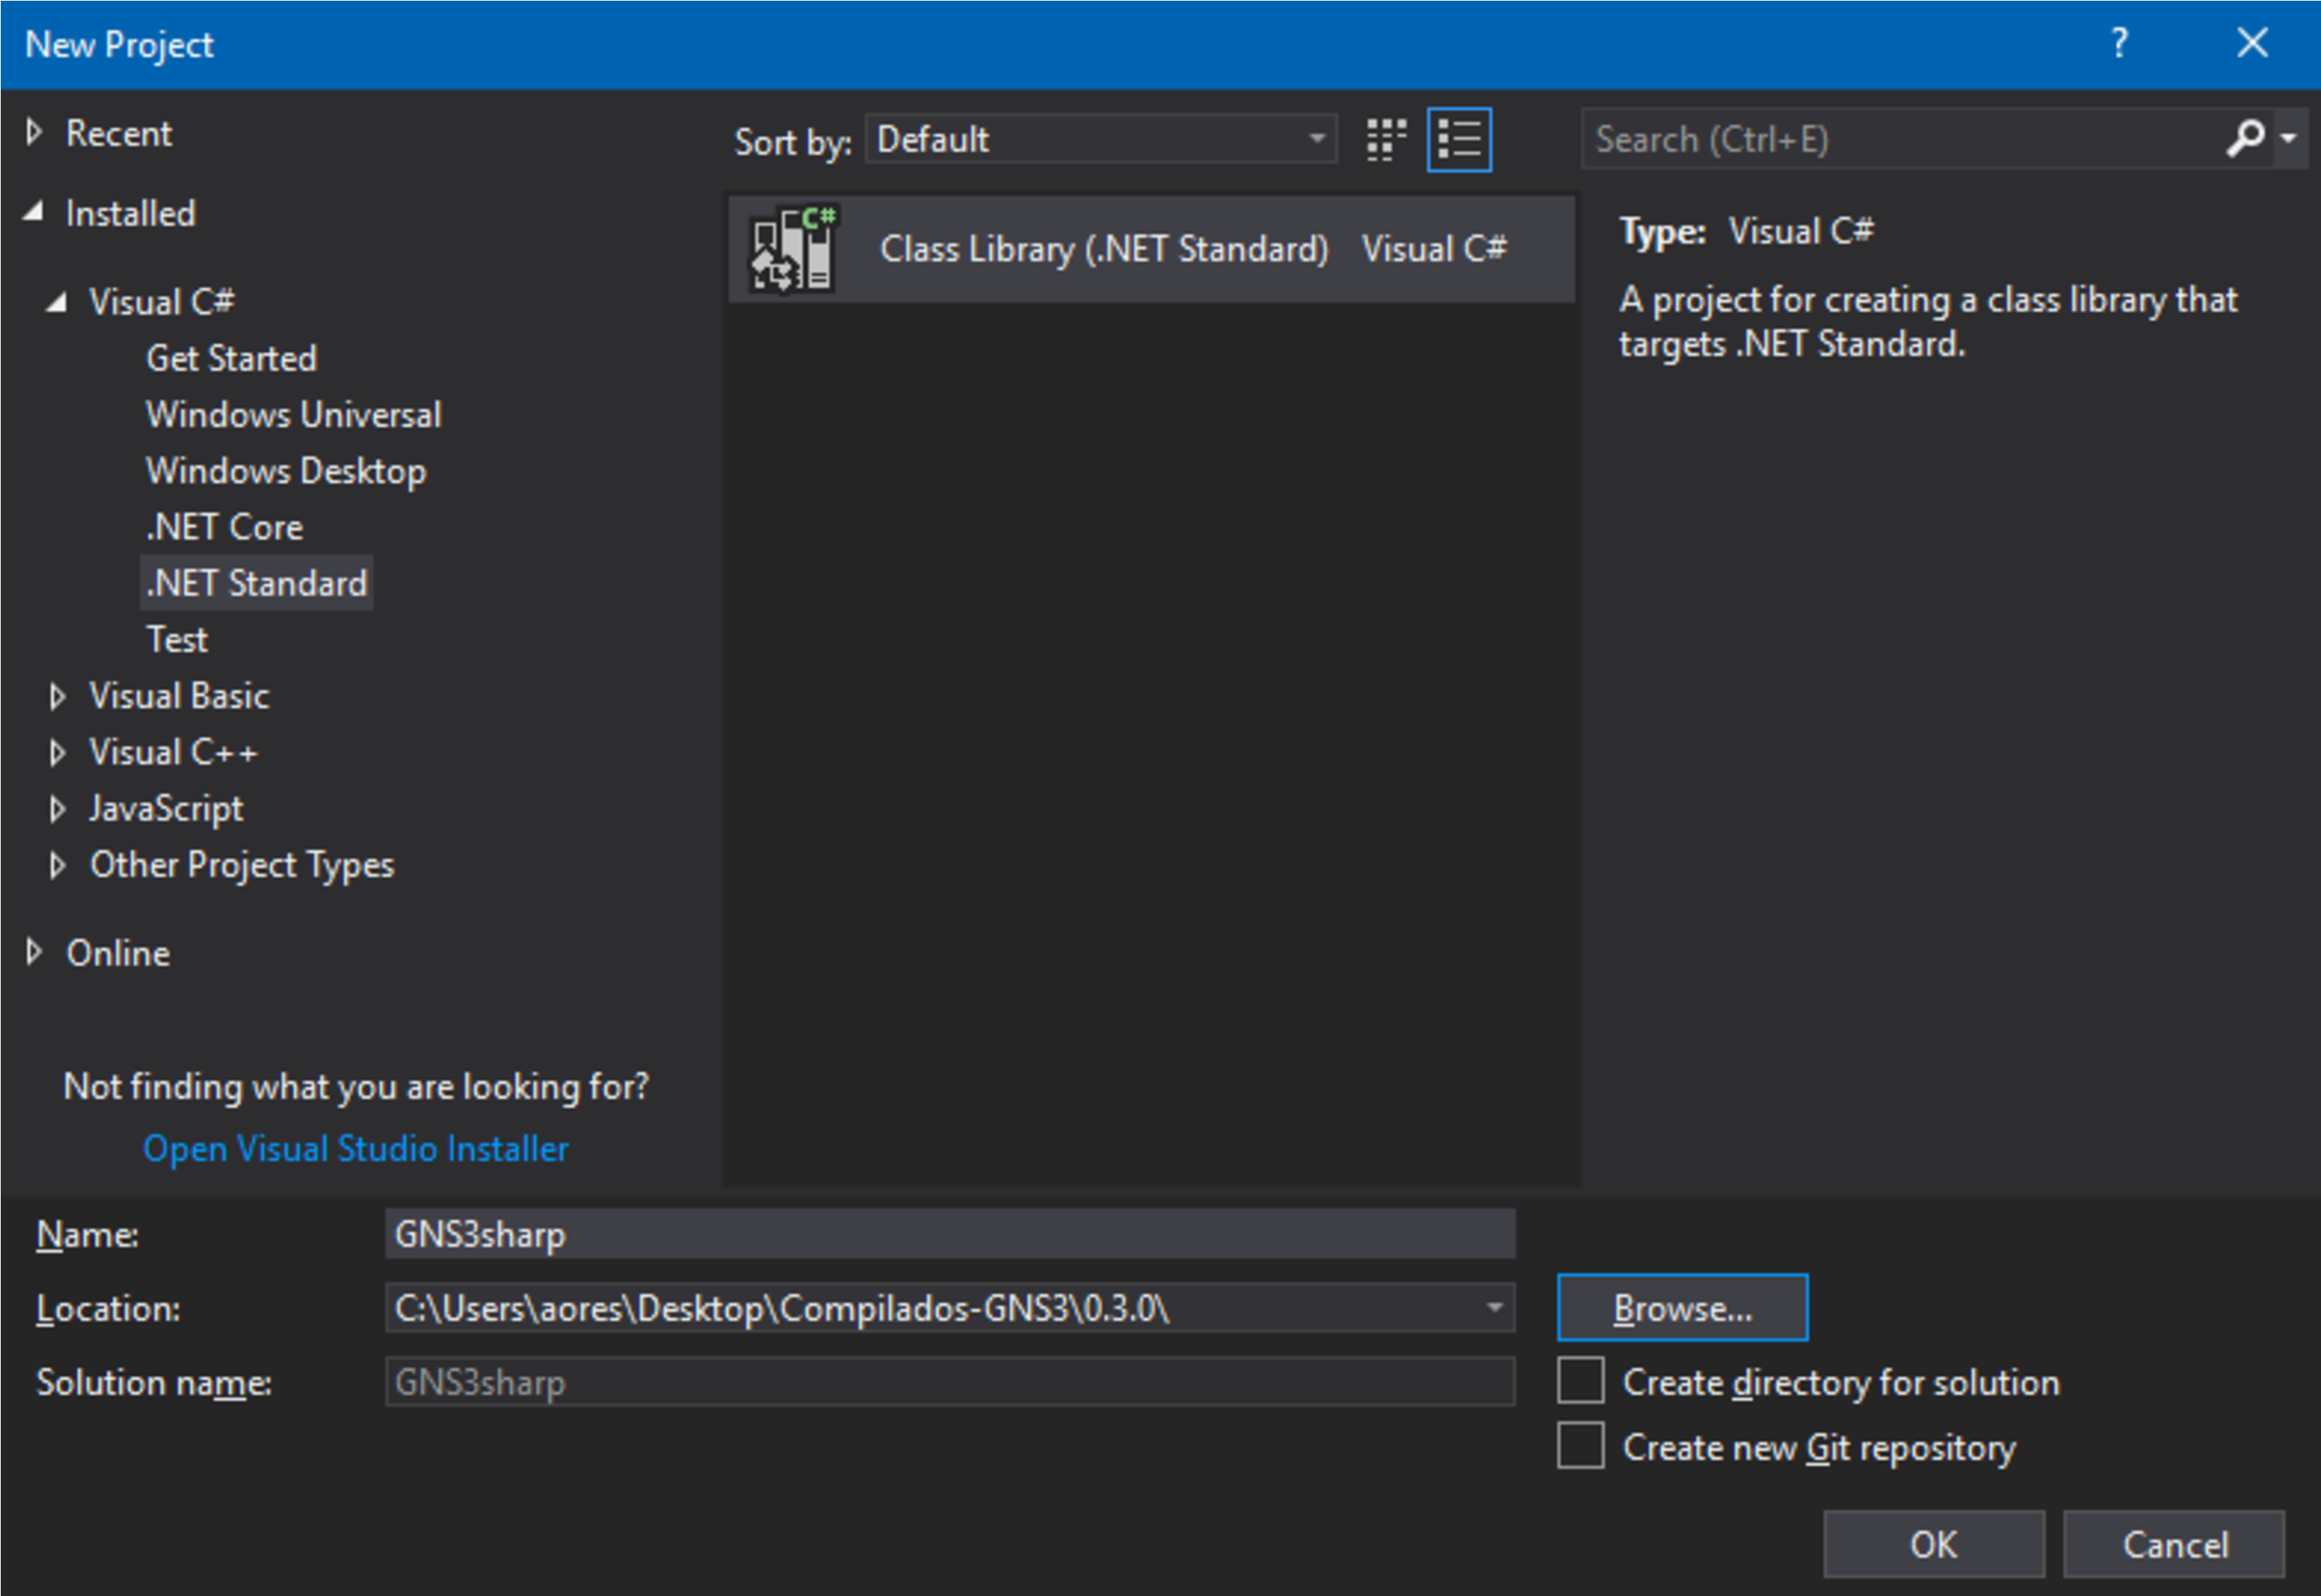
\includegraphics[scale=0.225]{imagenes/creacion_ensamblado}
  \caption{Elección del tipo de proyecto en Visual Studio 2017}
  \label{fig:creacion_ensamblado}
\end{figure}

Como framework con el que realizar la compilación se ha elegido \textit{.NET Standard 2.0}. De esta forma la librería será portable y correrá sin modificaciones en versiones modernas de todos los frameworks principales de .NET (.NET Core, .NET Framework...) pues únicamente posee el núcleo común de todos ellos. En realidad, .NET Standard no es un Framework: es simplemente una especificación que describe una base mínima de funcionalidad (tipos y miembros), que garantiza la compatibilidad con un cierto conjunto de frameworks.

Para el correcto ensamblado del código de la API hará falta la importación de dos librerías externas: \href{https://www.nuget.org/packages/Newtonsoft.Json/}{\textit{Json.NET}}, como ya se ha dicho en varias ocasiones, y \href{https://www.nuget.org/packages/Microsoft.CSharp/}{\textit{Microsoft.CSharp}}. Esta última, no incluida por defecto en .NET Standard, añade funcionalidades para la compilación dinámica de código (el modificador de acceso \texttt{dynamic} o el propio instanciador de clases por reflexión).

Con el fin de facilitar a los desarrolladores la importación de código de terceros, Visual Studio integra una herramienta que permite instalar esas dependencias en tus proyectos a través de \textit{NuGet}. NuGet es el formato de empaquetamiento de librerías de .NET para simplificar su compartición. Cuenta con una plataforma de hosting donde hospedar paquetes públicos paraser descrgados con facilidad por el resto de desarrolladores. La herramienta de Visual Studio se conecta directamente a este host, descarga el paquete y lo instala en el proyecto que esté siendo usado. Las dos librerías señaladas anteriormente se encuentran en tal plataforma.

Establecidos una serie de parámetros que servirán de metadatos para el ensamblado, se compila el proyecto. Visual Studio crea entonces el archivo \textit{.dll} así como un archivo \textit{.xml} que, enlazado al ensamblado, aporta la documentación de nuestra librería. Para lograr esto último fue necesario la inclusión de etiquetas XML como encabezado de cada uno elemento de la API (clases, métodos, propiedades...) cuya sintaxis puede \href{https://docs.microsoft.com/en-us/dotnet/csharp/programming-guide/xmldoc/xml-documentation-comments}{consultarse online}. Similar al Javadoc de Java.

Ya tenemos preparada la librería para que Unity haga uso de ella.

\subsection{GitHub y la comunidad}
Hemos considerado esencial que la API sea reutilizable. El objetivo de su desarrollo en ningún caso ha sido el de nacer y morir para el presente trabajo. Lejos de esto, se pretende que esta librería pueda ser utilizada por quien quiera, ya tenga como propósito la construcción de un videojuego o cualquier otra aplicación.

Con esto en mente, todo el código utilizado por la librería se encuentra disponible en \MYhref{https://github.com/aorestr/GNS3sharp}{este repositorio} de mi GitHub personal. Está liberado bajo una licencia MIT, tremendamente permisiva a la hora de reutilizar el código.

Además de los archivos de la propia API, se puede encontrar un README que explica algunos puntos importantes que considerar a la hora de utilizarla. En el repositorio de GitHub existe asimismo una sección de ``releases'', donde se suben los distintos compilados de la librería en formato ``.dll'' a medida que esta se expande o se reparan problemas aparecidos. Por supuesto, todo el código y su documentación están escritos en inglés para así llegar a más desarrolladores.


\section{Desarrollo del videojuego}
En esta sección se detalla la construcción del videojuego. En primer lugar se habla del juego en sí, qué se será creado y qué se puede esperar de la creación. Inmediatamente después se describe el entorno generado en GNS3 para ser usado por Unity para, más adelante, mostrar cómo y qué ha sido desarrollado mediante él.

\subsection{Descripción del juego}
Aunque al comienzo el propósito del proyecto era desarrollar algo similar a lo descrito en la subsección \ref{subsec:modelojuego}, en la subsección siguiente, la \ref{subsec:fracasojuego}, ya hablamos de la inviabilidad de la idea original. Propusimos entonces crear un pequeño nivel como prueba de concepto para así demostrar el potencial entre la biblioteca, el simulador y el motor de juego.

A modo de breve recordatorio sobre lo visto en aquella sección, el nivel será un pequeño escenario con varias plataformas. Cada una de estas hará simbólicamente de router. En ellas podrá encontrarse un cuadro mostrando la tabla de enrutamiento del nodo y una serie de puertas que hacen de sus interfaces. Al atravesarlas, se avanza hasta la plataforma que lleve al nodo que hay tras la interfaz. El objetivo es llegar hasta el aparato cuya IP aparece en la esquina inferior-izquierda de la pantalla.

\subsection{El proyecto de GNS3}
Para empezar será necesario construir la red sobre la que se apoyará el videojuego. Se ha construido una pequeña, de apenas cinco routers y dos PCs, uno como plataforma de inicio y otro como destino a alcanzar.

\begin{figure}[h]
  \centering
  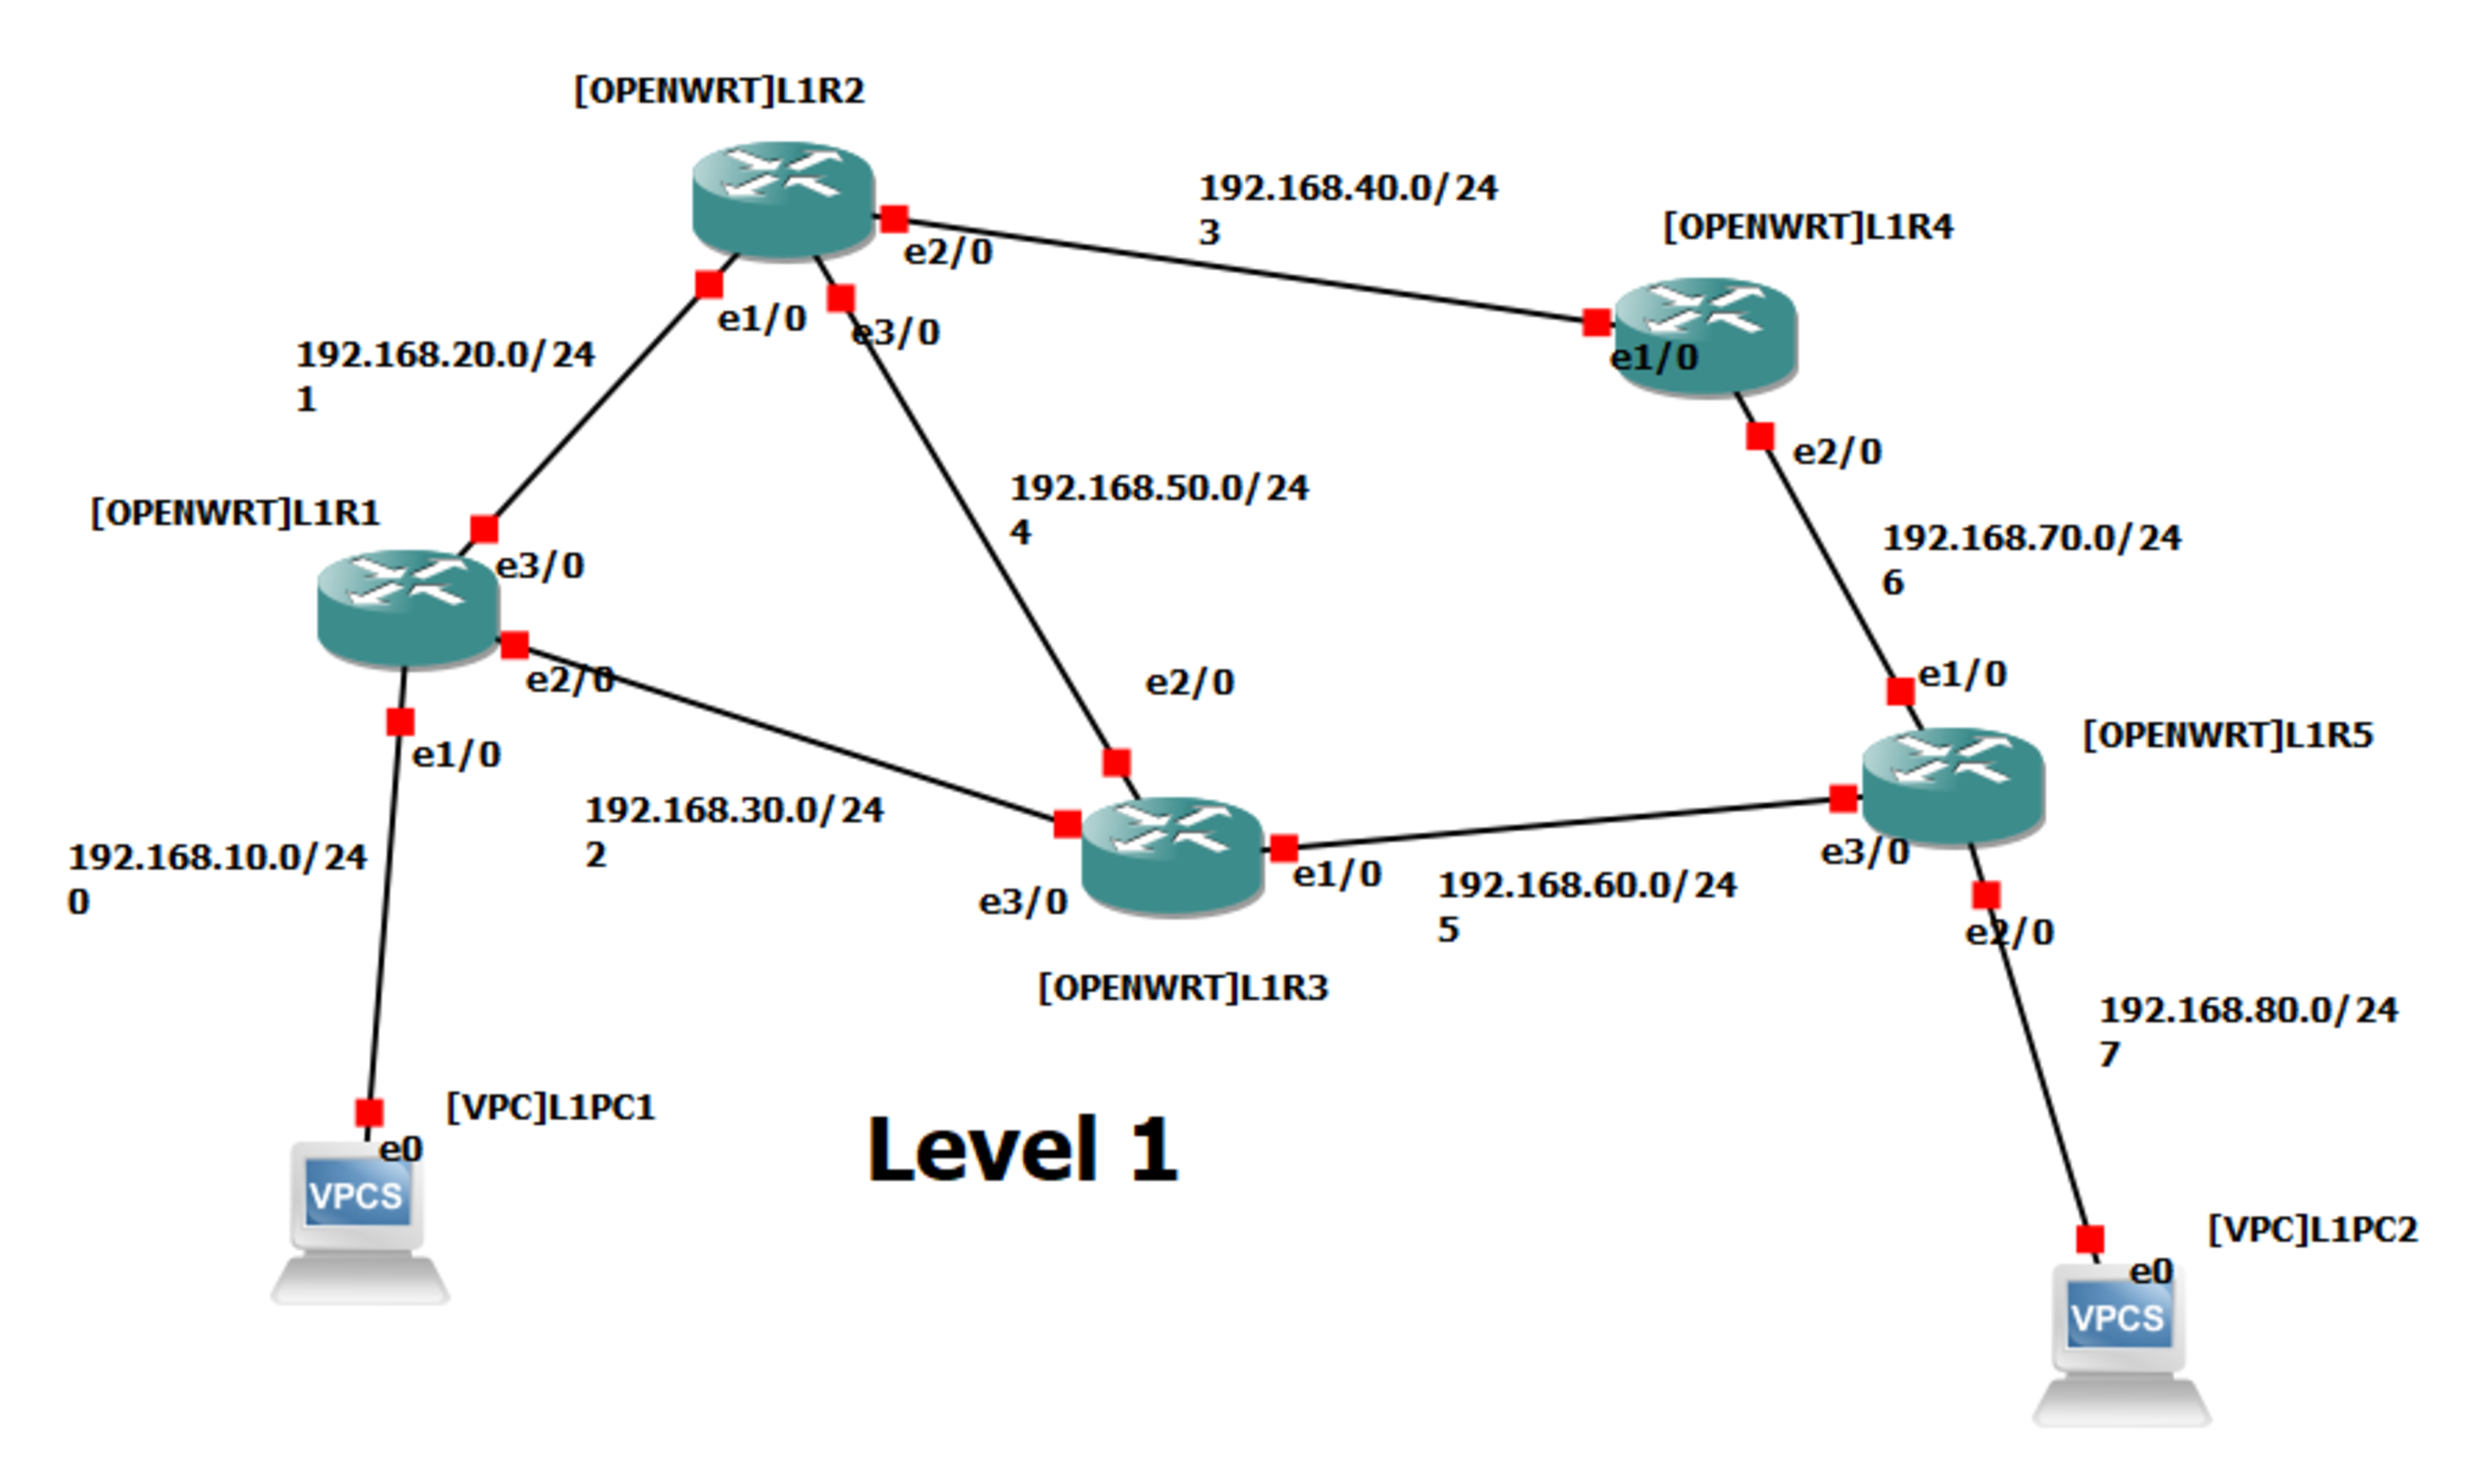
\includegraphics[scale=0.225]{imagenes/redGNS3}
  \caption{Red desplegada para el videojuego}
  \label{fig:esquematico_red}
\end{figure}

La figura \ref{fig:esquematico_red} está tomada directamente de la red desplegada en GNS3. Se comentarán a continuación los distintos aparatos usados y el modo en que han sido configurados.

\subsubsection{Dispositivos usados}
\begin{itemize}
\item \textbf{VPCs}: Los VPCs son unos de los pocos nodos interactivos que GNS3 incluye por defecto. Como su propio nombre indica, no son más que PCs virtuales que incluyen \textbf{funciones básicas} que se espera que un PC pueda usar en una red. Entre esas funciones está la de asignar una dirección a su interfaz y la de lanzar PINGs a través de ella. VPC es una gran herramienta para añadir hosts simples a GNS3 y probar la conectividad entre los nodos\cite{bookgns}.

Nuestra red cuenta con dos de ellos: \textit{[VPC]L1PC1} y \textit{[VPC]L1PC2}. Nótese la etiqueta con la que comienza su nombre, ya que como se comentó en anteriores ocasiones, esta sirve para que la API sea capaz de instanciar el objeto cuya clase representa este tipo de nodos (en este caso, la clase \texttt{VPC}). Solo consumen 2MB de RAM y la propia máquina anfitriona puede encargarse de gestionarlos (no es necesario pasar por GNS3 VM).

El único papel con el que cuentan estos dispositivos es el de representar mediante una dirección el inicio y el final del escenario.

\item \textbf{OpenWRT}: OpenWrt es una distribución GNU/Linux altamente extensible para dispositivos embebidos (típicamente routers inalámbricos). A diferencia de muchas otras distribuciones para estos routers, OpenWrt está construido desde cero para ser un sistema operativo completo y fácilmente modificable para el router. Esto significa que es posible tener todas las características que son necesarias en estos dispositivos con el añadido que corresponde a contar con un núcleo Linux\cite{aboutopenwrt}.

La principal razón por la que se eligió esta arquitectura como dispositivo de enrutamiento para el proyecto es su \textbf{gratuidad}: el proyecto OpenWRT es open source liberado bajo una licencia GPL. Debido a esto y a su filosofía de ``cada uno adapta su sistema operativo a sus propias necesidades particulares'', no se trata del firmware idóneo para un router al uso. Sin embargo, para nuestro propósito es más que suficiente.

Al estar basado en un sistema operativo Linux, gran parte de los comandos más famosos relacionados con redes como \texttt{ifconfig} aparecen aquí. Es un punto a su favor si conocemos tal arquitectura y las posibilidades que ofrece.

GNS3 cuenta con ``plantillas'' con las que se facilitar el importado de dispositivos como nodos a GNS3. Con el fin de incluir aparatos con OpenWRT instalado usamos la plantilla que puede descargarse desde \MYhref{https://www.gns3.com/marketplace/appliance/openwrt-2}{aquí}. Una vez descargada, siguiendo una serie de pasos GNS3 permite importar el nodo con mucha facilidad. La versión del firmware de OpenWRT que nosotros usamos es la 15.05.1. Slgo antigua considerando que data de 2016 y la última versión estable es la 18.06.1.

Todos los nodos que usen OpenWRT han de ser instalados en GNS3 VM si estamos trabajando desde Windows (en Linux no es necesario), pues el simulador no permite de ningún modo que la máquina anfitriona sea la encargada de gestionarlos. La mayor parte de los aparatos cuyas imágenes son de cierta complejidad como este están obligados a ser usados de este modo.

Cinco de estos dispositivos han sido desplegados en la red. El camino más rápido para cruzar del primer PC1 al PC2 sería, en condiciones normales, \textit{[OPENWRT]L1R1} $\rightarrow$ \textit{[OPENWRT]L1R3} $\rightarrow$ \textit{[OPENWRT]L1R5}.

Las redes que han sido marcadas en los enlaces de la figura \ref{fig:esquematico_red} son únicamente orientativas ya que, como se explicará en el apartado siguiente, se ha pseudo-aleatorizado el establecimiento de estas. De nuevo, atención a \textit{[OPENWRT]} en el nombre de los routers: es la etiqueta asociada a la clase \texttt{OpenWRT} para que \GNSCS~pueda instanciar el objeto apropiado.

\item Otros dispositivos que consideramos añadir pero que, finalmente, por la simplicidad del diseño no se incluyeron, son el switch multicapa \MYhref{https://www.openvswitch.org/}{\textbf{Open vSwitch}} y la variante de Tiny Core, distro Linux altamente modular, \MYhref{https://docs.gns3.com/appliances/microcore-linux.html}{\textbf{Micro Core}}. Ambos son dispositivos de uso libre y gratuito, de ahí nuestro interés por ellos.
\end{itemize}

Antes de pasar a la siguiente sección, es necesario aclarar que el prefijo ``L1'' del nombre de todos los nodos hace referencia a ``Level 1''. Se da a entender por consiguiente que el proyecto parte de la idea de que los nodos de todos los niveles pasaran a estar en el mismo esquemático.

\subsubsection{Despliegue}
Los dispositivos se han interconectado tal y como se aprecia en la ilustración \ref{fig:esquematico_red}. Ninguno de los enlaces cuenta con tipo alguno de filtro, con lo que se consideran ideales.

Por sencillez, todas las redes establecidas en el despliegue tiene máscara de red de 24 bits. Todas ellas son de la forma \texttt{192.168.x0.y}, donde \texttt{x} es un número que se aleatoriza con cada arranque del juego mediante programación (hablaremos de esto cuando se detalle el apartado técnico de construcción del mismo) e \texttt{y} el número asociado a la interfaz del dispositivo que está conectada a esa red. Así, como ejemplo y suponiendo que las redes de la figura citada son las definitivas, a la interfaz de arriba de L1R1 (\texttt{eth3}) se le asignaría la dirección \texttt{192.168.20.3}. En el caso de los PCs, \texttt{y} sera en ambos casos \texttt{11}.

Al arrancar la red (al inicializar cada nodo), los VPCs son funcionales casi inmediatamente. No obstante, no es el caso en absoluto de los routers. Al tratarse de dispositivos que emulan aparatos reales, con un sistema operativo de cierta envergadura, es necesario \textbf{esperar para que su arranque sea completo}. Así, los nodos con OpenWRT necesitan varios minutos para ser completamente funcionales en el PC desde el que se han realizado las pruebas. Esto implica que, o bien se ha de tomar la precaución de que todos los dispositivos estén iniciados al comenzar el juego, o bien que el jugador ha de esperar el tiempo necesario para que los aparatos comiencen a estar disponibles.

La problemática pasa a ser doble, ya que \textbf{GNS3 no guarda el estado de las máquinas tras su apagado}. Por más información que se ha buscado para intentar paliar este inconveniente, nada parece ser efectivo. La consecuencia natural es, por consiguiente, que el dispositivo habrá de ser configurado cada vez que se reinicie. Este no es un problema per se, pues gracias a la API puede llevarse a cabo mediante unas líneas de código con total facilidad; el verdadero problema es que, aún así, configurar todas las interfaces de un proyecto lleva tiempo. El tiempo podría ser minimizado si cada router es configurado paralelamente.

Todo lo anterior se resume en:
\begin{enumerate}
\item La asignación de direcciones se aleatoriza gracias a las posibilidades de scripting de la API.
\item Los routers requieren de un cierto tiempo de arranque, en absoluto inmediato, para ser completamente funcionales.
\item La configuración de los dispositivos es descartada cada vez que son apagados, con lo que es necesario reconfigurarlos tras cada arranque. Esto lleva implícito una inevitable inversión de tiempo.
\end{enumerate}

\subsection{El proyecto de Unity}
En esta sección se describe tanto el diseño del nivel de nuestro juego como el proceso que se ha seguido para materializarlo. Se comenzará señalando los materiales que han posibilitado la construcción del escenario.

\subsubsection{Materiales}
\begin{itemize}
\item El fondo es una imagen estática tomada de \MYhref{https://opengameart.org/content/industrial-background-2d}{OpenGameArt}, una famosa web que publica arte redistribuible para la elaboración de juegos. Está liberado bajo una licencia	\href{CC 3.0}{https://creativecommons.org/licenses/by/3.0/}, lo que implica que puede ser compartido y copiado siempre y cuando se dé crédito al autor y una referencia al material. Un enlace desde donde puede ser encontrado ya se ha dejado en la línea anterior. Gracias a ``Alucard'' por esta imagen.
\item El decorado del nivel se ha generado gracias a un conjunto de sprites localizados una vez más en \MYhref{https://opengameart.org/content/sci-fi-platform-tiles}{OpenGameArt}. En esta ocasión, el material tiene licencia \href{https://creativecommons.org/publicdomain/zero/1.0/}{CC0 1.0}, de dominio público; totalmente libre.

Un sprite es más un mapa de bits usado como elemento individual cuyo conjunto posibilita crear escenas en un videojuego. Si atendemos a esa definición y reparamos en la imagen a la que puede accederse desde el enlace anterior, es evidente que esa descripción no se corresponde a la figura. Digamos que esa imagen está formada por decenas de pequeños sprites y es tarea nuestra el extraerlos para nuestro propio uso. Unity nos lo pone fácil, ya que contiene una herramienta llamada ``sprite editor'' (visible en la figura \ref{fig:sprite_editor}), que disecciona imágenes para convertirlas en pequeñas piezas. Si los sprites están repartidos con un tamaño fijo en la imagen, como es nuestro caso, es tan sencillo como indicarle tal dimensiones en píxeles y Unity hará el resto.

\begin{figure}[h]
  \centering
  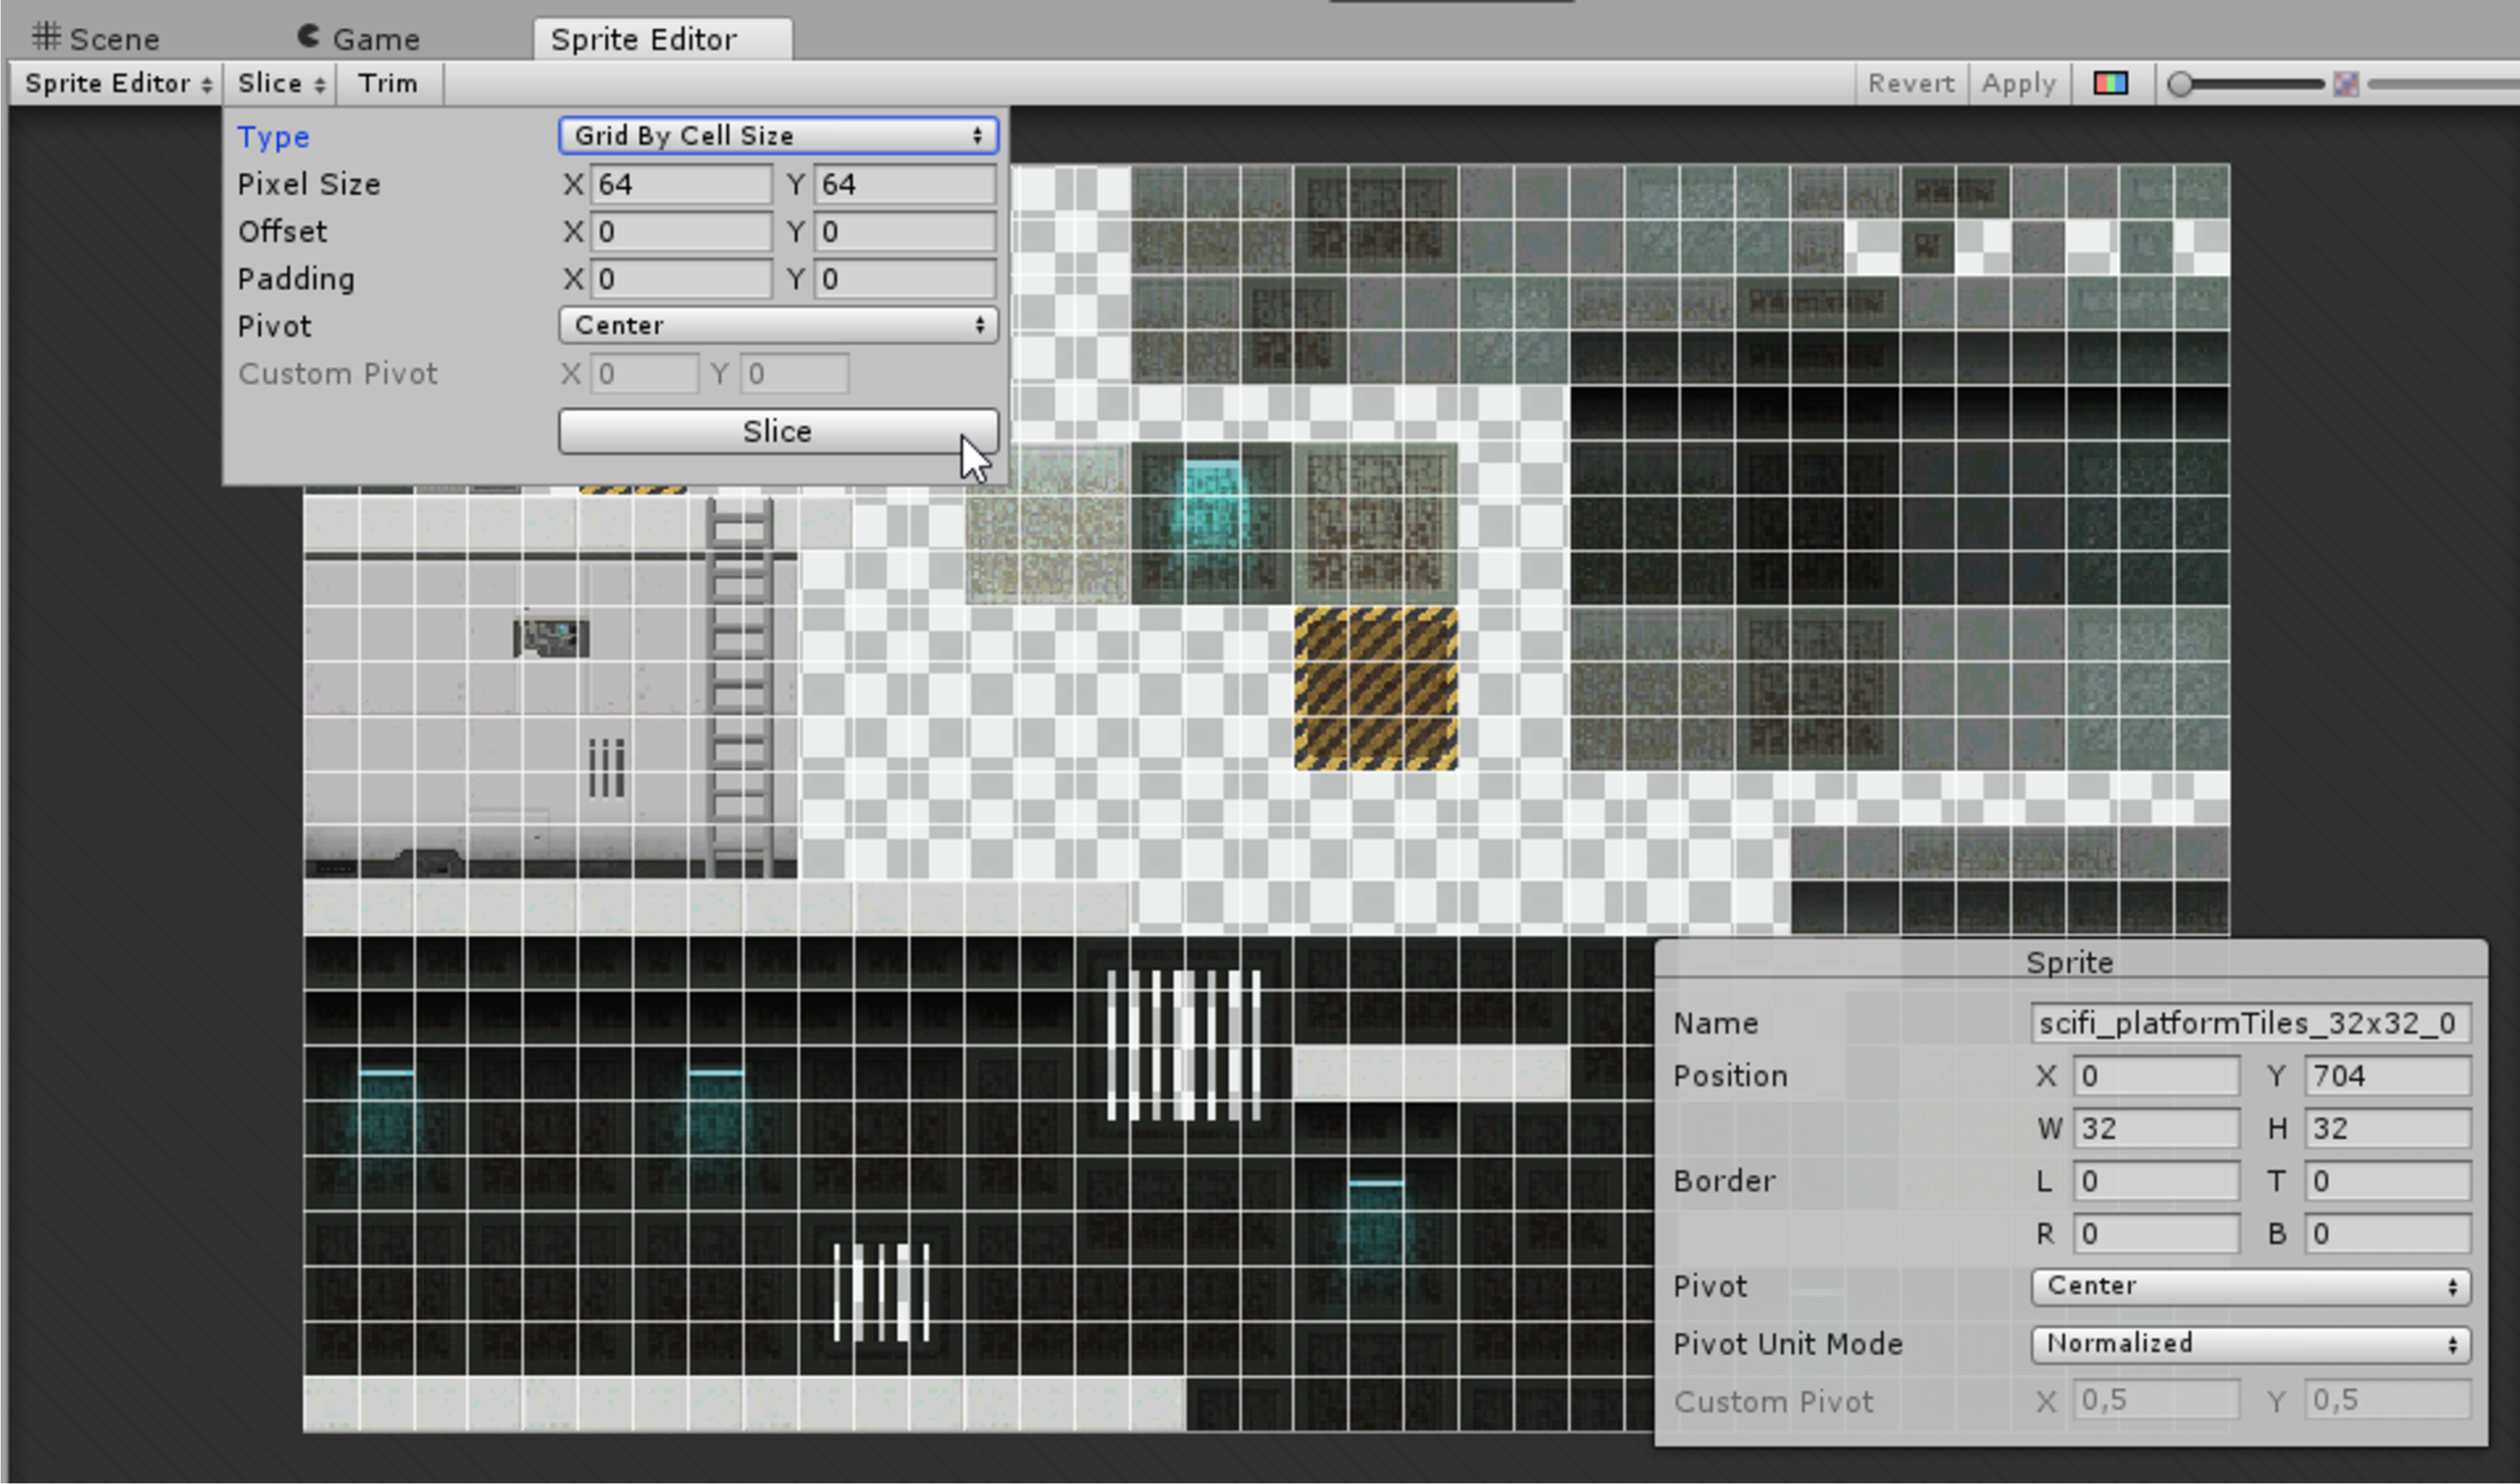
\includegraphics[scale=0.175]{imagenes/sprite_editor}
  \caption{Editor de sprites de Unity}
  \label{fig:sprite_editor}
\end{figure}

Ya veremos de qué modo son usados los sprites en el siguiente apartado.

\item Finalmente, nos hemos visto ayudados por uno de los paquetes que Unity incluye por defecto. Se trata del paquete ``2D'', que puede ser descargado desde el propio cliente de Unity en \textit{Assets} $\rightarrow$ \textit{Import package} $\rightarrow$ \textit{2D}. Incluye una serie de assets (\textbf{ESTE CONCEPTO DEBE EXPLICARSE LA PRIMERA VEZ QUE SE HABLE DE UNITY}) básicos para la creación de niveles bidimensionales. 

\end{itemize}

\subsubsection{Objetos del juego}
El juego cuenta con, únicamente, dos escenas. La primera, aquella que aparece justo al ser inicializado, consta de únicamente una interfaz de usuario (GUI) que pide al jugador que pulse ``espacio'' para comenzar a jugar. Al hacerlo, se configura toda la red de GNS3 que pudimos ver en la figura \ref{fig:esquematico_red}. Todo el aspecto relacionado con la programación podrá estudiarse en el punto siguiente.

Pasado un tiempo, después de que todo quede configurado, Unity toma los datos necesarios del proyecto de GNS3 para construir la siguiente escena, la principal.

\begin{figure}[h]
  \centering
  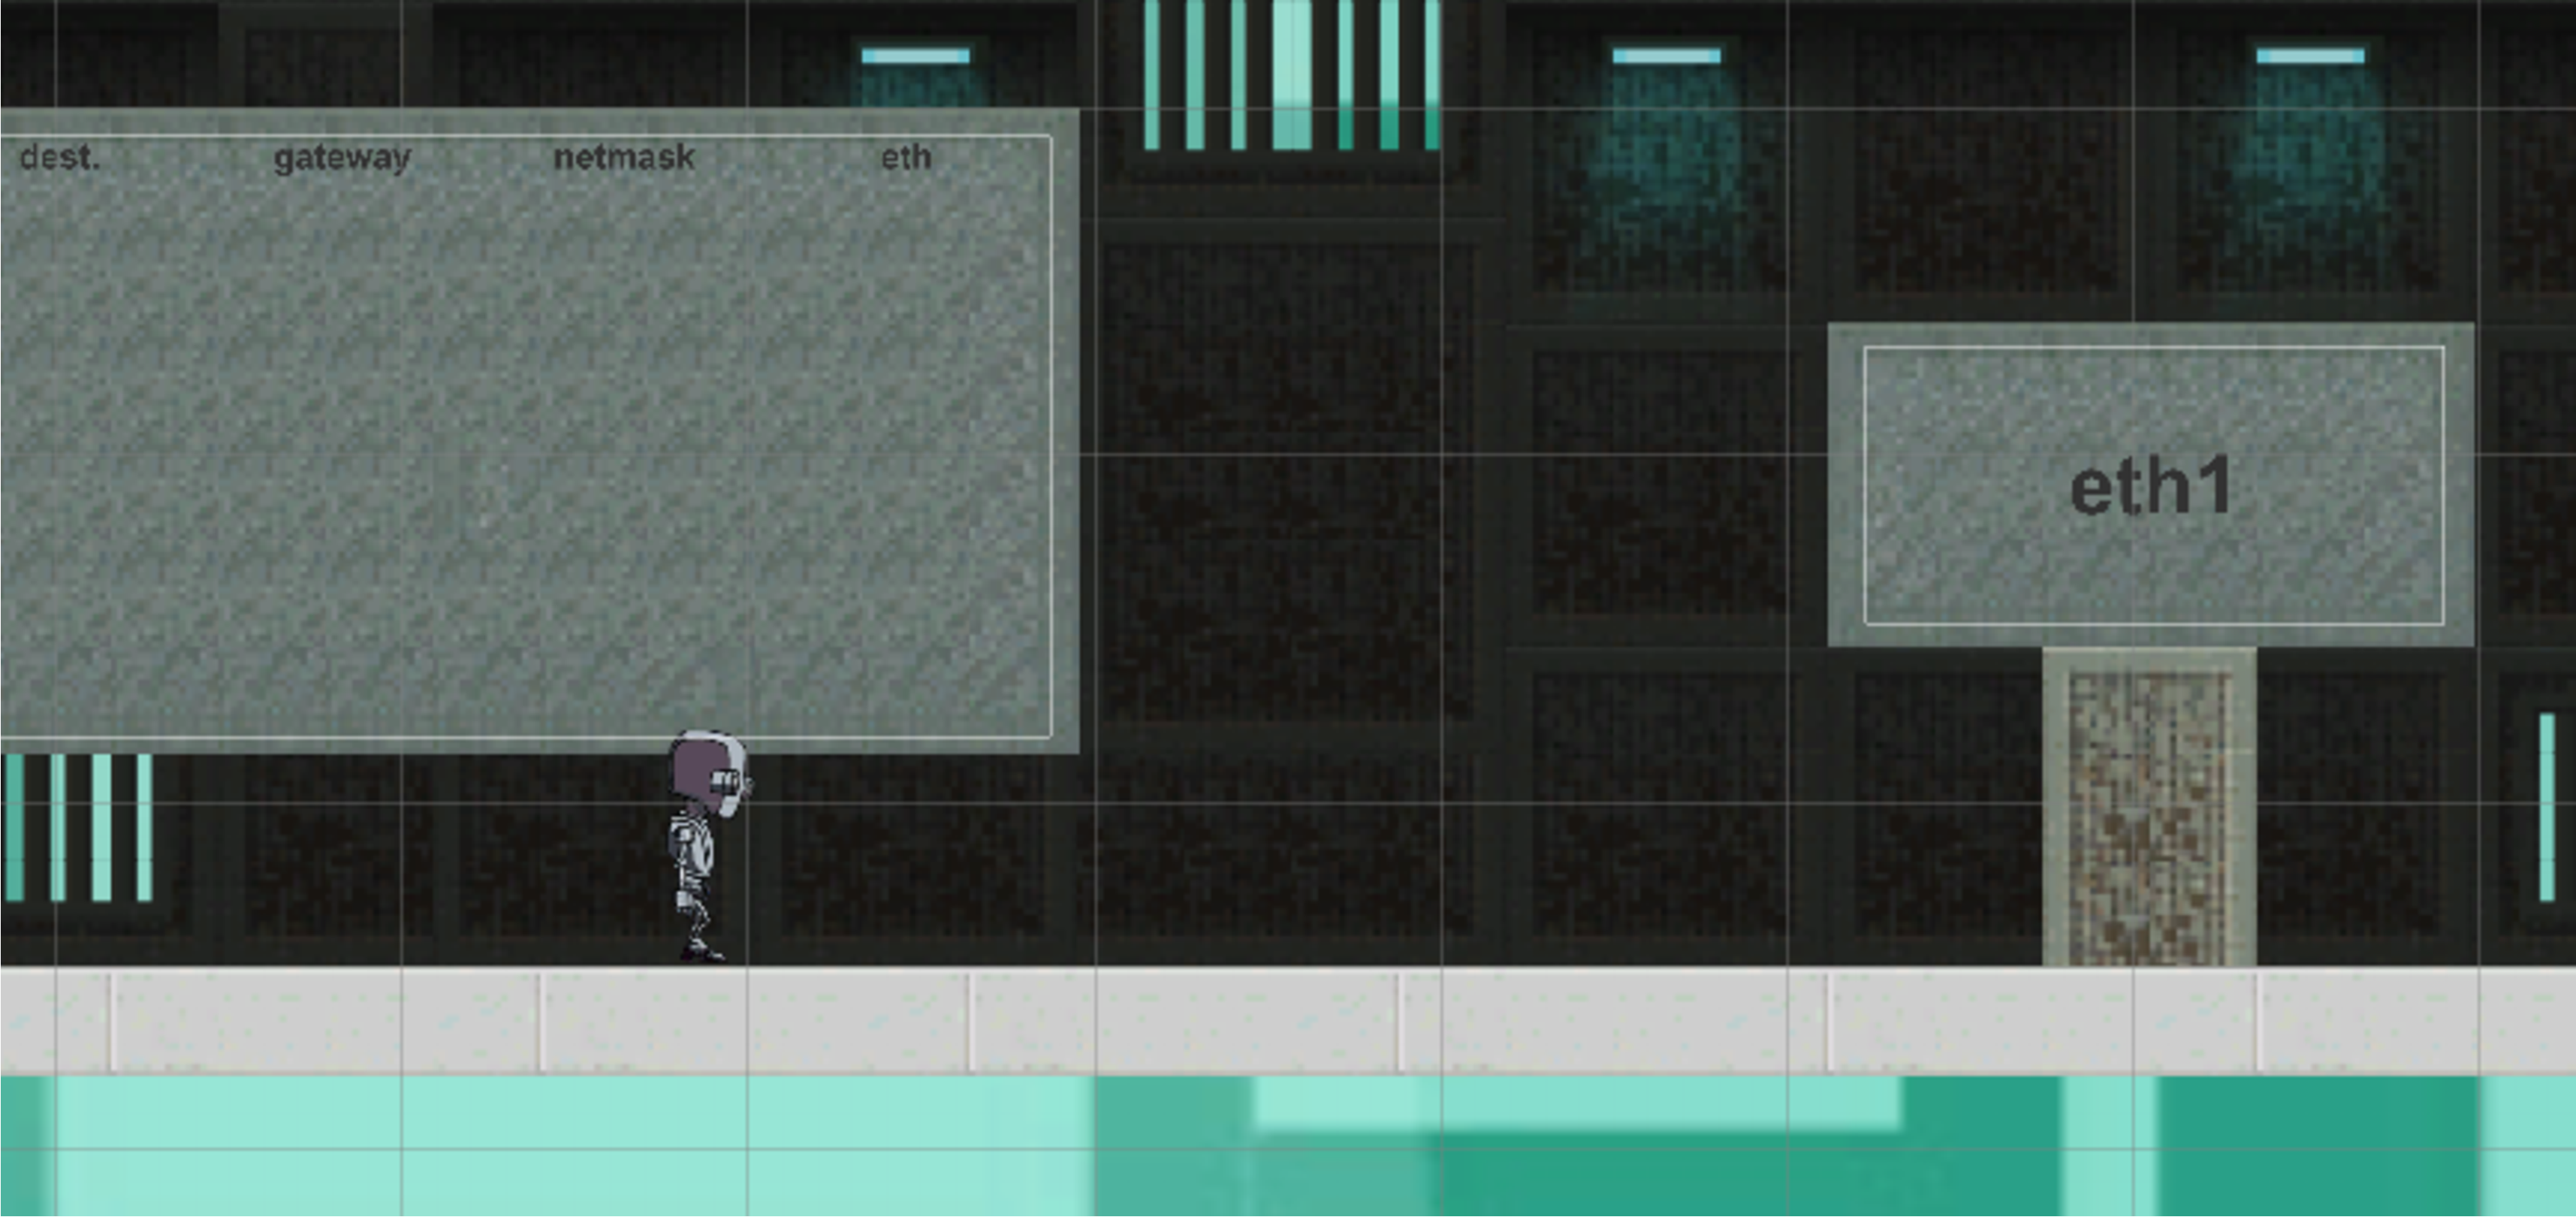
\includegraphics[scale=0.175]{imagenes/monieco}
  \caption{Plataforma del nivel del juego}
  \label{fig:monieco}
\end{figure}

En la figura \ref{fig:monieco} pueden apreciarse los elementos más importantes del escenario:

\begin{itemize}
\item Por un lado \textbf{el protagonista}, el objeto sobre el que el jugador tiene poder. Se controla como en cualquier juego de plataformas bidimensional (crucetas para moverse, espacio para saltar...). El personaje es uno de los assets que el paquete ``2D'' trae consigo, con lo que no fue necesario ningún tipo de programación adicional. Cuenta con físicas ya definidas a través de un elemento \texttt{Rigidbody 2D} (deja a un objeto bajo el control del motor de físicas de Unity\cite{rigidbody}) y un par de elementos collider (definen la forma de un objeto para las colisiones físicas\cite{colliders}).
\item Las \textbf{paredes} del escenario están construidas con sprites procesados como ``tiles''. Los tiles son objetos que permiten a un sprite ser renderizado en un ``tilemap''\cite{tiles}. Los tilemaps son, a su vez, una redecilla de cuadrículas donde se permite la inserción de estos tiles. Todo esto no es más que una herramienta que facilita la creación de niveles. 
\item El \textbf{suelo} del escenario también está formado por tiles. Sin embargo, la diferencia con los anteriores reside en que el tilemap sobre el que están montados contiene un elemento adicional: consta de un \texttt{Tilemap Collider 2D}. Este elemento otorga automáticamente físicas de colisión a todos los tiles que incluyamos en el tilemap. Ello significa que todo tile introducido en el tilemap desplegado colisionará con el protagonista, permitiendo a este moverse sobre él.
\item Las \textbf{puertas} son la representación de las interfaces de los routers en el videojuego. Llevan a un nodo o a otro. Son, de nuevo, tiles, sobre los que se han dispuesto objetos vacíos que únicamente tienen un \texttt{Box Collider 2D} como elemento integrado. Posee un ``trigger'' (disparados) que manda una señal cada vez que un objeto colisiona con él.
\item Los carteles de las \textbf{tablas de encaminamiento}. Necesitan ser llenados con la información que se extraiga directamente de los routers.
\item Además, y aunque en la imagen no pueda ser apreciada, tenemos la cámara principal del juego, que rige lo que ve el jugador en todo momento. El objeto que la representa cuenta con un script predefinido en el paquete ``2D'' que permite seguir automáticamente a un objeto de la escena. Se ha elegido a protagonista como objeto que la cámara debe encargarse de seguir.
\end{itemize}

Para terminar este apartado, se facilita una vista más general del escenario en la figura \ref{fig:nivel}, donde pueden observarse las distintas plataformas que lo conforman.

\begin{figure}[h]
  \centering
  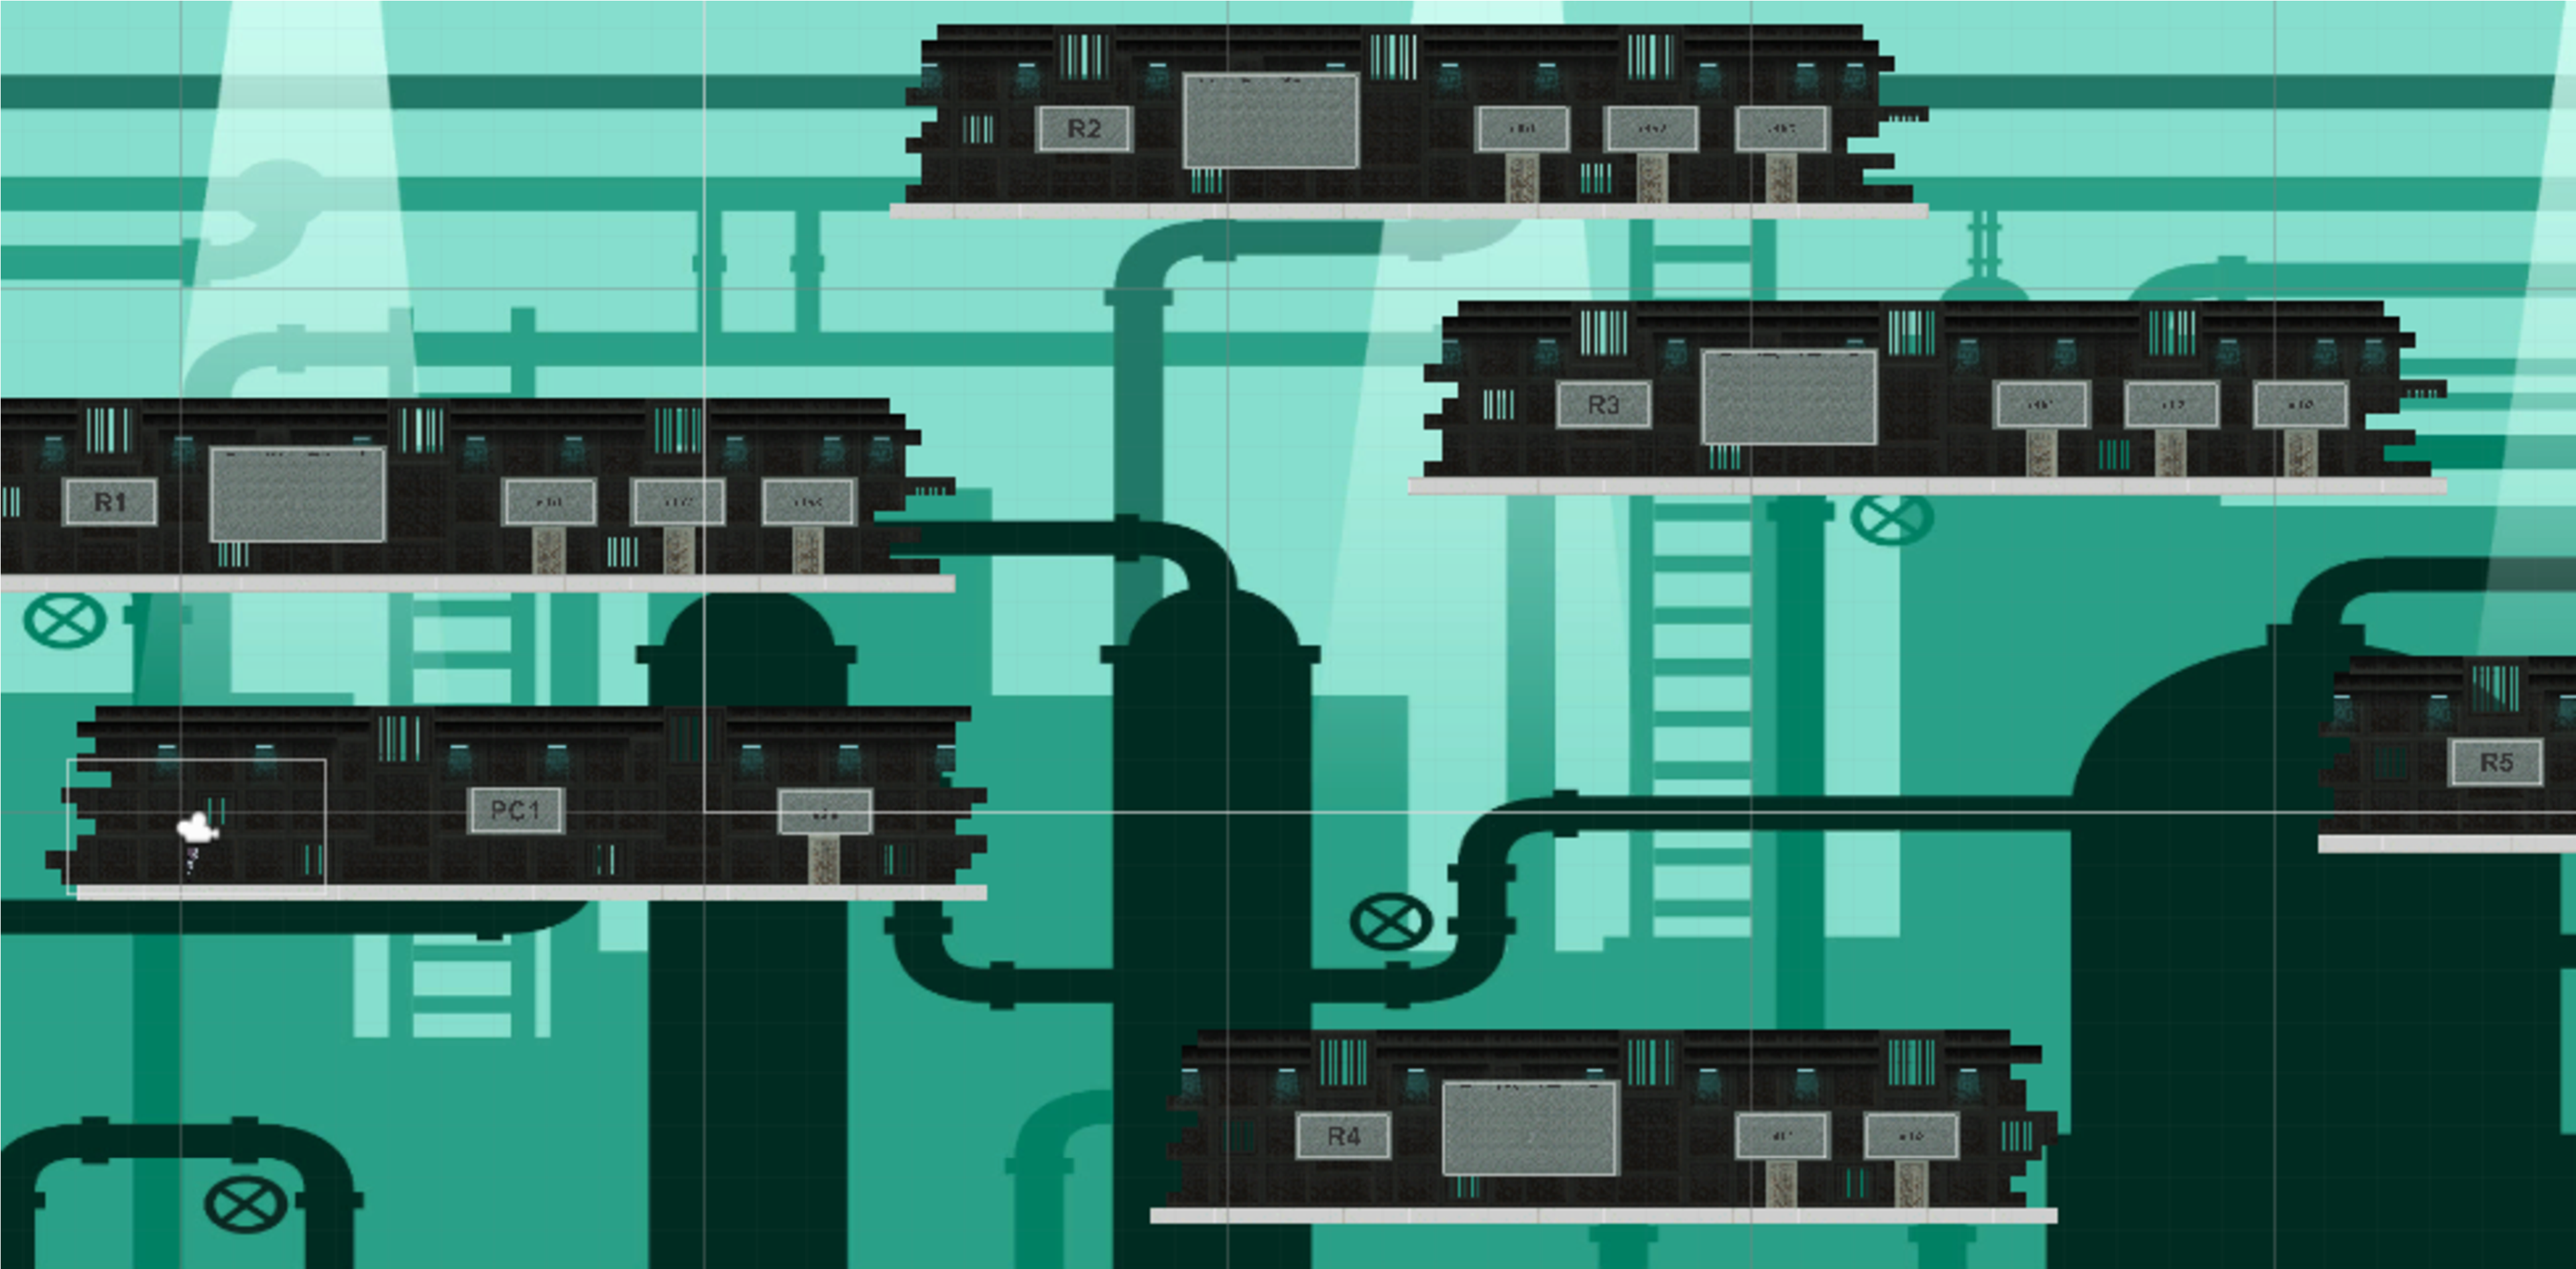
\includegraphics[scale=0.175]{imagenes/nivel}
  \caption{Escenario creado}
  \label{fig:nivel}
\end{figure}

\subsubsection{Scripting}
El \textit{scripting} de un videojuego no es más que la programación que existe en él para llevar a cabo toda la lógica que lo rige. Describiremos a continuación los distintos scripts que han sido utilizados para posibilitar el funcionamiento del juego.

Para que estos puedan hacer uso de la librería que hemos desarrollado, hace falta depositar el \texttt{.dll} de la misma (y el \texttt{.xml} con la documentación que se generó junto a él) junto al de las dependencias que vimos en la subsección \ref{subsec:compilation} en la carpeta ``Assets'' del proyecto de Unity. Esta carpeta aparece en todo proyecto y contiene, como su propio nombre indica, todos los elementos o assets de los que el juego se valdrá. Con el fin de que Unity procese correctamente la información del ensamblado, se requiere configurar las preferencias del proyecto para que este haga uso de .NET 4.x como motor de ejecutado de los scripts y de .NET Standard 2.0 como nivel de compatibilidad de API.

\begin{itemize}
\item \texttt{GNS3Handler}: crea y guarda una instancia de \GNSCS~para ser utilizada por todos los objetos de la escena que la necesiten. Como no queremos que cada elemento de la escena instancie un objeto de esta clase (es un gasto de recursos innecesario), haremos que sea ``singleton''. En programación, un singleton es una clase que tan solo permite que \textbf{una instancia} de sí misma sea creada\cite{csindepth}. Para llevarlo a cabo, cada vez que se intente instanciar la clase, se comprobará si su propiedad estática \texttt{Instance} contiene información. En caso negativo, se crea el objeto; en caso contrario, se destruye el objeto de la escena desde el que se ha intentado instanciar la clase.

\begin{lstlisting}[language={[Sharp]C}, caption={\texttt{GNS3Handler}}, label={GNS3Handler_code}]
using UnityEngine;

public class GNS3Handler : MonoBehaviour {

    public static GNS3Handler Instance { get; private set; } = null;
    public GNS3sharp.GNS3sharp projectHandler;

    // Awake is always called before any Start function
    void Awake() {
        if (Instance == null) {
            Instance = this;
            this.projectHandler = new GNS3sharp.GNS3sharp(
                GNS3sharp.ServerProjects.GetProjectIDByName("GameNet")
            );
        }
        else if (Instance != this)  Destroy(gameObject);
    }

}
\end{lstlisting}

El script es colocado en la primera escena. Al arrancar esta, se instancia un objeto de la clase \GNSCS, el cual solicita al servidor de GNS3 información acerca de un proyecto denominado ``GameNet'' (es como fue llamado el proyecto que contiene la red ya vista) para ser gestionado. Dada la simpleza del juego, no se ha creído conveniente habilitar mecanismos de control de errores, entendiendo por estos problemas a la hora de encontrar el proyecto solicitado, etc.

\item \texttt{L1Mapping}: esta clase define una serie de propiedades y métodos estáticos que son de ayuda para otras clases de la escena. Nació como un baúl donde guardar variables necesarias para ciertos elementos de la escena.

\begin{itemize}
\item \texttt{L1Mapping.NodeNamesM1}: siguiendo la filosofía recién citada, guarda una cadena de \texttt{string}s con los nombres de los nodos que pueden encontrarse. Con ``L1'' nos referimos al nivel y con el ``M1'' al minijuego o fase dentro del mismo. Dado que no ha sido desarrollada más que una escena, esta sintaxis cae en desuso.
\item \texttt{L1Mapping.NodeRespawnM1}: para ir de una plataforma a otra del nivel el personaje es teletransportado. Esta propiedad guarda un mapeo entre cada una de las plataformas-nodos y la posición del mapa en la que el personaje debe reaparecer al acceder a cada una de ellas.
\item \texttt{L1Mapping.DoorsOrderM1}: aleatoriza el orden de las puertas-interfaces de cada plataforma, logrando de esta manera que cambie a cada partida.
\item \texttt{L1Mapping.RandomizeNets()}: aleatoriza la \texttt{x} de redes del tipo \texttt{192.168.x0.y}; redes como las que usamos en nuestro nivel. Así, la configuración de la red varía también a cada ejecución del programa.
\begin{lstlisting}[language={[Sharp]C}, caption={\texttt{L1Mapping.RandomizeNets()}}, label={RandomizeNets_code}]
public static ushort[] RandomizeNets(ushort numLinks)
{
    // Result list
    List<ushort> tempLinks = new List<ushort>(numLinks);
    // Initial list
    List<ushort> initialList = new List<ushort>(numLinks);
    // Random variable
    System.Random rnd = new System.Random();

    for (ushort i = 10; i <= numLinks * 10; i += 10) initialList.Add(i);
    for (ushort i = 0; i < numLinks; i++)
    {
        // Pick a random net number (10, 20, 30...) from the list
        var randIdx = rnd.Next(0, initialList.Count);
        tempLinks.Add(initialList[randIdx]);
        initialList.RemoveAt(randIdx);
    }
    return tempLinks.ToArray();
}
\end{lstlisting}
\end{itemize}

\item \texttt{L1M1Handler}: contiene la mayor parte de la lógica del nivel y, por tanto, ha de cargarse al comienzo de la escena. Inicializa todos los nodos del proyecto de GNS3 asociados al nivel, asigna variables con las referencias de cada uno de ellos y espera cuatro minutos a que todos ellos finalicen su arranque. Tras ello, configura los dispositivos del proyecto, comenzando por los PCs y continuando por los routers. El código del que se dispone a continuación muestra parte del proceso:

\begin{lstlisting}[language={[Sharp]C}, caption={\texttt{L1M1HandlerHelper.SetUpRouters()} y \texttt{L1M1HandlerHelper.SetUpRouters()}}, label={L1M1HandlerHelper_code}]
public static void SetUpRouters(OpenWRT[] Routers, ushort[] NetsPrefix) {
    Task[] tasks = new Task[5]
    {
        Task.Factory.StartNew(() => SetUpR1(Routers[0], NetsPrefix)),
        Task.Factory.StartNew(() => SetUpR2(Routers[1], NetsPrefix)),
        Task.Factory.StartNew(() => SetUpR3(Routers[2], NetsPrefix)),
        Task.Factory.StartNew(() => SetUpR4(Routers[3], NetsPrefix)),
        Task.Factory.StartNew(() => SetUpR5(Routers[4], NetsPrefix))
    };
    Task.WaitAll(tasks);
}

private static void SetUpR1(OpenWRT R, ushort[] NetsPrefix) {
    // Net interfaces
    R.ActivateInterface(IP: $"192.168.{NetsPrefix[0]}.1", interfaceNumber: 1, netmask: "255.255.255.0");
    R.ActivateInterface(IP: $"192.168.{NetsPrefix[2]}.2", interfaceNumber: 2, netmask: "255.255.255.0");
    R.ActivateInterface(IP: $"192.168.{NetsPrefix[1]}.3", interfaceNumber: 3, netmask: "255.255.255.0");
    R.DisableFirewall();
    // Routes
    R.SetRoute(destination: $"192.168.{NetsPrefix[7]}.0", gateway: $"192.168.{NetsPrefix[2]}.3", netmask: "255.255.255.0");
    R.SetRoute(destination: $"192.168.{NetsPrefix[5]}.0", gateway: $"192.168.{NetsPrefix[2]}.3", netmask: "255.255.255.0");
    R.SetRoute(destination: $"192.168.{NetsPrefix[3]}.0", gateway: $"192.168.{NetsPrefix[1]}.1", netmask: "255.255.255.0");
    R.SetRoute(destination: $"192.168.{NetsPrefix[4]}.0", gateway: $"192.168.{NetsPrefix[2]}.3", netmask: "255.255.255.0");
    R.SetRoute(destination: $"192.168.{NetsPrefix[6]}.0", gateway: $"192.168.{NetsPrefix[1]}.1", netmask: "255.255.255.0");
}
\end{lstlisting}

Los dos métodos mostrados forman parte de \texttt{L1M1HandlerHelper}, una clase contenida dentro de \texttt{L1M1Handler} con algunas funciones que esta necesita. Tal como puede intuirse en las líneas de \texttt{SetUpRouters()}, se ha paralelizado la configuración de los routers, reduciendo drásticamente el tiempo de inicio del nivel. Esto se lleva a cabo mediante la clase predefinida de C\# \texttt{Task}, que permite la definición de tareas ejecutadas en hilos independientes.

Existe una tarea para la configuración de cada router, llevada a cabo con funciones como \texttt{SetUpR1()}.

Finalmente, \texttt{L1M1Handler} también se encarga de cosas como el dibujado de las tablas de enturamiento en el nivel y la creación de un contador ascendente que se muestra continuamente en pantalla. La finalidad de este último es la de incentivar al jugador a terminar el mapa en el menor tiempo posible. De haberse desarrollado más el juego, habría cobrado más sentido, con elementos como bases de datos donde guardar las puntuaciones de cada partida.

\item \texttt{DoorOrder}: tiene como misión asignar el cartel que habrá encima de cada puerta así como determinar cuál será la posición en la que reaparezca el protagonista cuando decida atravesar una de ellas.

El script es insertado en unos \texttt{GameObject}s utilizados para representar las puertas en la escena, permitiéndole a aquel tomar parámetros personalizados de cada una de ellas. Así, conociendo el número de la puerta y la plataforma-nodo en la que reside, mediante \texttt{L1Mapping} puede averiguar fácilmente cuál es la interfaz asociada a ella y cuál es la posición que el personaje obtendrá una vez decida atravesarla.

Como el cartel ubicado encima de cada puerta marcará la IP asociada a la interfaz del nodo correspondiente, es necesario buscar el modo de recibirla. La forma de hacerlo podría ``trampearse'' a través de alguno de los mapeos de \texttt{L1Mapping}, pero se ha decidido llevarlo a cabo mediante el método \texttt{OpenWrt.GetIPByInterface()}, que extrae la información a través de una consulta al router. La problemática asociada a esta solución es el tiempo que requiere, pues ha de hacerse por cada puerta y no es en absoluto un proceso automático.

\item Otras clases de menor calibre que no nos detendremos a explicar son:
\begin{itemize}
\item \texttt{EscToExit}: permite que al pulsar ``Esc'' se salga del juego.
\item \texttt{ExistLevel}: cierra el juego al llegar a la plataforma-PC final.
\item \texttt{FallDown}: devuelve al personaje a una zona segura si se cae de alguna plataforma.
\item \texttt{Teletransport}: desplaza la posición del personaje hasta unas ciertas coordenadas del escenario.
\item \texttt{SceneLoader}: se incrusta en la primera escena y carga desde ella la segunda. El script esta tomado directamente de otra persona, a la que se da crédito en el propio código.
\end{itemize}

\end{itemize}

%
%\chapter{Pruebas}\label{chap:Pruebas}

fgxdh

\section{Descripción del problema}

huigk




%
%\chapter{Conclusiones}\label{chap:Conclusiones}
Antes de finalizar el documento, recordaremos los puntos claves de lo que se pudo leer en él en relación al proyecto y haremos una valoración global del mismo.

\section{Trabajo realizado}
Hemos comenzado el proyecto hablando de los beneficios educativos de los videojuegos y cómo pretendemos usarlos trayéndolos al área de la telemática. Para ello nos hemos válido de un software de virtualización de redes con la intención de integrarlo en el juego. Sin embargo, la interacción entre simulador de redes y juego requiere de trabajo previo.

La parte del proyecto que le es relativa describe con todo detalle el método llevado a cabo para volver interactiva una red virtualizada a través de una herramienta externa a ella. La red virtualizada es generada mediante el simulador GNS3. La susodicha herramienta, por su parte, se materializó en una librería para el lenguaje C\#. Para llevar a cabo la biblioteca, se requiere el uso de la API REST de GNS3, desde la cual mandamos peticiones, tanto en busca de información como a la espera de crear cambios en la red.  Es asimismo necesario crear conexiones con los nodos contenidos en los proyectos con sockets, gracias a los cuales ganamos total control sobre ellos. La biblioteca nos permite desde encender y apagar dispositivos por la red, pasando por crear nuevos enlaces entre ellos, hasta controlarlos de forma absoluta. Las posibilidades son amplias.

Tras ello, pasamos a la creación de un juego. Insertando la biblioteca desarrollada en los entresijos del videojuego somos capaces de controlar todo lo que ocurre en la red virtualizada. Esto tiene repercusión bilateral: el juego puede nutrirse de la la red, de sus estructura y de su información, a la vez que puede modificarla tal y como sea necesario.

A través de la utilidad, se creó un pequeño ``puzzle'' cuyas indicaciones eran extraídas directamente desde la red virtual. El puzzle pone a prueba los conocimientos de enrutamiento del jugador mediante un sencillo laberinto, donde cada plataforma del nivel remite a un router de la red el cual permite el salto al siguiente mediante una serie de puertas que no simbolizan otra cosa que las interfaces de cada uno.

Finalmente, durante las pruebas del proyecto, se propuso una configuración alternativa del simulador de redes. En lugar de ser instalado de forma nativa, es enteramente desplegado en una máquina virtual que, al ser exportada en un formato fácilmente importable en un hipervisor, facilita la portabilidad de las redes y, por consiguiente, de los juegos que sean desarrollados junto a ellas. Esta evaluación de las alternativas de despliegue del juego se llevó a cabo a través de la medida de valores como el consumo de RAM y  el tiempo de arranque de ambas alternativas. Se concluyó que aunque la configuración relativa a la máquina virtual es levemente inferior en cuanto a rendimiento, sus beneficios la hacen más interesante.

\section{Valoración del resultado}
La API desarrollada puede suponer una herramienta de gran utilidad para aplicaciones de un gran número de áreas en el mundo de la telemática. Al haber sido cuidada de forma tan detallada, su utilización e incluso modificación posterior no posee complejidad alguna. Afirmamos que, en este sentido, un éxito. Nos hemos encargado de que exista información suficiente para aquel que pretenda retomarla mediante documentación tanto en el código como en el repositorio donde este se hospeda.

Existen problemas que aún no hemos podido resolver con éxito en la librería. La mayor parte de las veces son problemas, no directamente de la API, sino del propio simulador. Pongamos por caso uno de los más problemáticos: el arranque de cada dispositivo. Si el aparato en concreto es pesado, GNS3 necesita de un tiempo del orden de minutos para que sea satisfactoriamente iniciado, lo que implica un retraso para cualquiera que sea la aplicación desde la que se esté lanzando la librería. Además, esta aún no ha encontrado el modo de automatizar la comprobación de la operatividad de un nodo para comenzar a trabajar con él. Es necesario entones escribir una sentencia de pausa en la aplicación, lo cual es rudimentario y poco preciso y por ende implica fallos en potencia.

Pese a todo ello la librería es plenamente funcional. Tiene limitaciones como el no poder generar proyectos de GNS3 desde cero o su dependencia con aquel programa, que necesita ser inicializado previamente de forma manual (no se ha automatizado su arranque) para poder trabajar con él.

Posiblemente el verdadero punto débil del proyecto haya sido el videojuego. Y es que aunque al comienzo se pretendía llevar a cabo un juego completo que explotará la API al máximo y que fuera capaz de explicar varias asignaturas de la telemática, finalmente se optó por crear algo mucho más pequeño. El desarrollo de un videojuego completo es una tarea de gran complejidad que requiere de un número de horas mucho mayor del que era viable dedicar a este proyecto. Para adaptarse a las circunstancias, la decisión tomada fue la de crear un solo nivel que demostrase que la interacción con la biblioteca es funcional. El resultado pudo verse en el capítulo \ref{chap:Pruebas}.

Si bien efectivamente se comprobó la viabilidad de la relación GNS3$\leftrightarrow$API$\leftrightarrow$Juego, quizá no fuera explotada lo suficiente. Muchas de las características insertadas en la librería han quedado excluidas del juego final pues no son útiles para el mismo. Añadir nuevos niveles habría garantizado su inclusión en el mismo, pero ello también implicaba una planificación más detenida y un mayor desembolso temporal inviable.

En cualquiera de los casos, como ha quedado demostrado en el documento, el proyecto ha estado centrado en la interacción entre los distintos elementos de nuestro problema. Se trata de una prueba de concepto que, consideramos, ha sido fructuosa.

\section{Experiencia personal}
El desarrollo de este proyecto ha supuesto un aprendizaje continuo para mí. He descubierto qué son los simuladores de redes, me he introducido en el mundo de la programación de videojuegos, he aprendido a C\# y a trabajar en el entorno .NET... y realmente un largo número de etcéteras más. Ha sido realmente una experiencia plena porque todo ese aprendizaje provenía de uno mismo: de las constantes batallas contra los problemas aparecidos y de la habilidad para resolverlos con los medios dados.

Por un lado me siento plenamente satisfecho con el trabajo realizado, pues he abierto un camino sobre el que firmemente pienso que es importante seguir trabajando. Me apena saber que el videojuego que tenía en mente cuando comencé el proyecto no haya podido llevarse a cabo. Mi nula experiencia con motores de juegos me ha ralentizado enormemente a la hora de crear. Esto se traduce en grandes cantidades de tiempo invertidas en pasos elementales y pequeños, reduciendo considerablemente el número de horas para el desarrollo de algo más grande.

\section{Trabajo futuro}
Tal y como se ha repetido en varias ocasiones, la API ha sido creada de forma que cualquier nuevo desarrollador que pretende hacer uso de ella, lo tenga fácil para ello. Así, proponemos que más adelante el proyecto sea retomado. 

Existen, como es de suponer, mejoras posibles en la biblioteca. Así por ejemplo, establecida una conexión con los nodos, cada envío y recepción de mensajes lleva un tiempo. 

Como el presente trabajo se ha propuesto y ha logrado crear la interacción entre el videojuego y la red virtualizada, la persona que encargada de reiniciarlo tendría la responsabilidad de completar lo relativo al videojuego. Este traspaso de testigo consistiría en construir un videojuego de ciertas dimensiones que ponga en práctica lo teorizado durante el documento; algo como lo que podíamos ver en la sección \ref{subsec:modelojuego}. Utilizar todas aquellas funciones que no fueron implementadas en este; aprovechar mejor la biblioteca y sus posibilidades. Disponible la herramienta y las indicaciones necesarias para hacerlo, solo queda ponerlas en práctica.
%
%%\chapter{Conclusiones y Trabajos Futuros}
%
%
\nocite{*}
\bibliographystyle{unsrt}
\bibliography{bibliografia/bibliografia}

%\appendix
%\input{apendices/manual_usuario/manual_usuario}
%%\input{apendices/paper/paper}
%\input{glosario/entradas_glosario}
% \addcontentsline{toc}{chapter}{Glosario}
% \printglossary
\chapter*{}
\thispagestyle{empty}

\end{document}
